% !TEX root = ./main.tex
\documentclass[UTF8, 10pt]{ctexart}
\usepackage[
    a4paper,
    left=0.5cm,
    right=0.5cm,
    top=1.0cm,
    bottom=1.0cm,
    columnsep=0.5cm]{geometry}
\usepackage{amssymb,amsmath, bbm, amsthm, mathrsfs}
\usepackage{graphicx}
\usepackage{caption}
\usepackage{subcaption}
\usepackage{xcolor}
\usepackage[colorlinks,linkcolor=violet]{hyperref}
\usepackage{titlesec}
\usepackage{tabularx}
\usepackage{booktabs}
\usepackage{float}
\usepackage{multicol}

\titleformat{\section}
    {\normalfont\Large\bfseries\filright}
    {\thesection}
    {1em}
    {}

\setlength{\floatsep}{0pt plus 1pt minus 1pt}
\setlength{\textfloatsep}{0pt plus 1pt minus 1pt}
\setlength{\intextsep}{0pt plus 1pt minus 1pt}
\titlespacing*{\section}{0pt}{*0}{*0}
\titlespacing*{\subsection}{0pt}{*0}{*0}

\newcommand{\textor}{\,\text{or}\,}
\newcommand{\textand}{\,\text{and}\,}
\DeclareMathOperator{\nullable}{nullable}
\DeclareMathOperator{\first}{First}
\DeclareMathOperator{\follow}{Follow}

\date{}
\title{编译原理 Compiler Principle}

\begin{document}

\maketitle
\vspace*{-25mm}
\begin{multicols}{2}
% ======================================================
\section{Lexical Analysis}
\label{section:lexical-analysis}
% !TEX root = ./main.tex
% Lexical Analysis
% ======================================================
\subsection*{正则表达式和形式语言}
\par \noindent 形式语言的运算:给定语言 $L=\{a, b\}, M = \{cc, dd\}$:
\par \noindent $L \cup M = \{s | s\in L \textor s \in M\} =  \{a, b, cc, dd\}$
\par \noindent $LM = \{st | s\in L \textand t \in M\} = \{acc, add, bcc, bdd\}$
\par \noindent $L^0 = \{\varepsilon\},L^1 = L, L^n = L^{n-1}L^n$
\par \noindent $L^* = L^0 \cup L^1 \cup L^2 \cup \dots$(Kleene 闭包)
\par \noindent $L^+ = L^1 \cup L^2 \cup L^3 \cup \dots$(正闭包)
\par \noindent 运算的优先级:闭包\texttt{*} > 连接 > 选择\texttt{|}
\par \noindent 正则表达式 $r$ 定义正则语言,记为 $L(r)$,正则语言 $L(r), L(s)$:
\par \noindent $L(r|s) = L(r) \cup L(s)$、$L(rs) = L(r)L(s)$、
\par \noindent $L(r^*) = (L(r))^*$、$(L(r)) = (Lr)$
\par \noindent 正则表达式满足运算定律:\texttt{|} 可交换、可结合。连接可结合,对\texttt{|} 可分配。闭包满足幂等性 $r^{**} = r^*$。
\par \noindent FA 无法计数,正则表达式不能用于描述配对或嵌套的结构。
\begin{figure}[H]
    \centering
    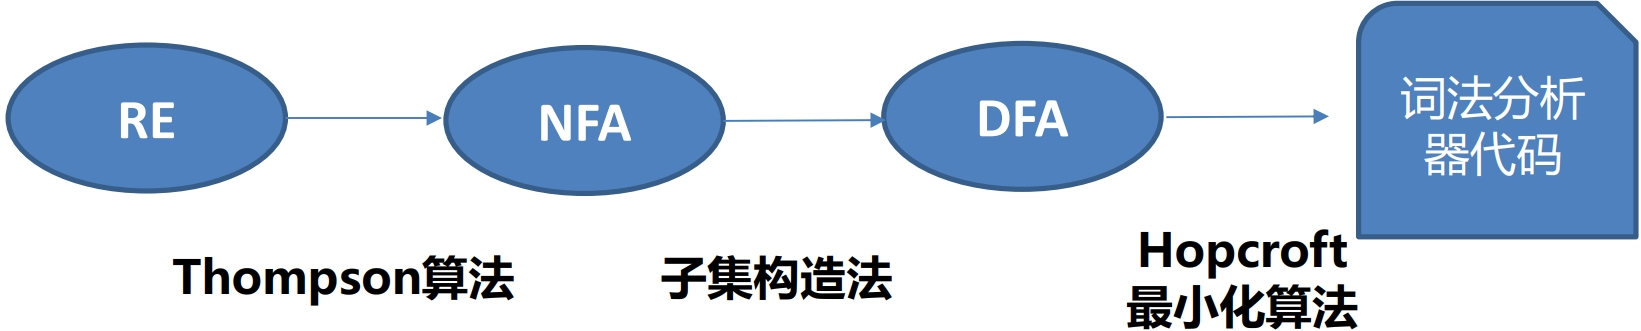
\includegraphics[width=0.8\linewidth]{figures/lex1.png}
\end{figure}
\par \noindent RE $\rightarrow$ NFA:结构归纳法。
\begin{figure}[H]
    \centering
    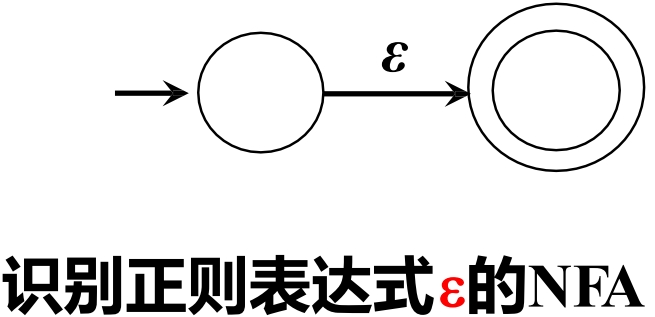
\includegraphics[width=0.3\linewidth]{figures/lex2.png}
    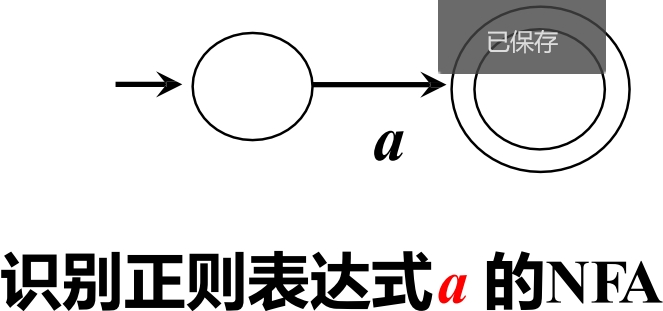
\includegraphics[width=0.3\linewidth]{figures/lex3.png}
    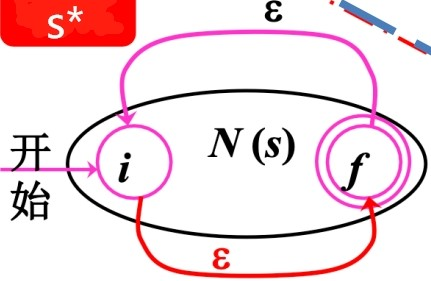
\includegraphics[width=0.2\linewidth]{figures/lex6.png}
\end{figure}
\begin{figure}[H]
    \centering
    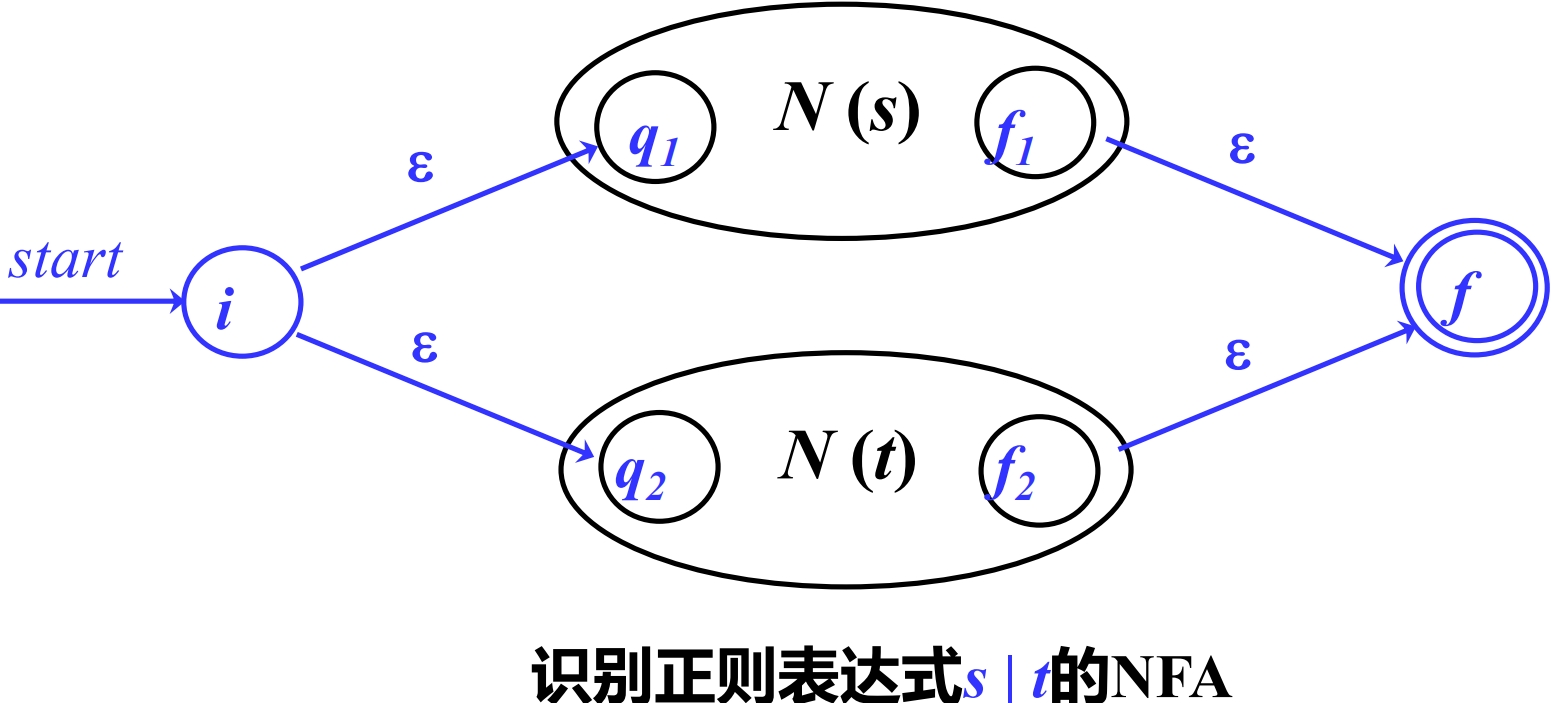
\includegraphics[width=0.4\linewidth]{figures/lex4.png}
    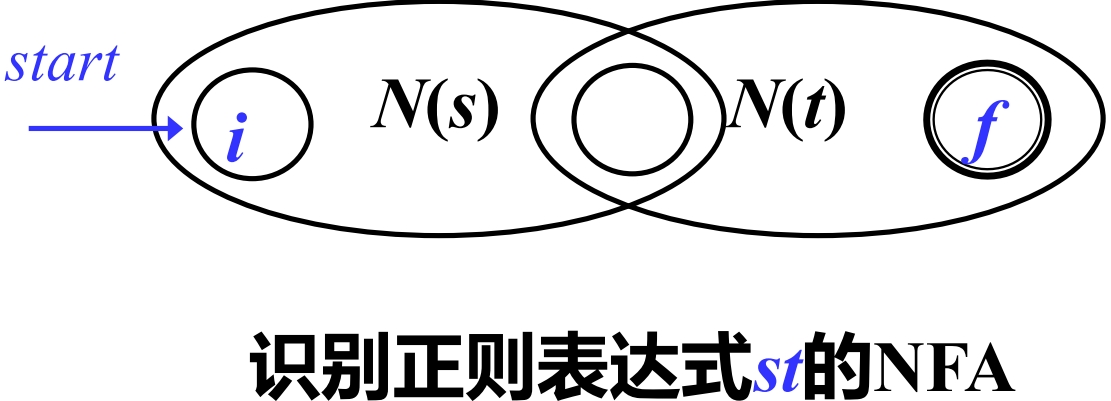
\includegraphics[width=0.4\linewidth]{figures/lex5.png}
\end{figure}
\par \noindent NFA $\rightarrow$ DFA:子集构造法。
\par \noindent NFA 的初始状态的 e-闭包 对应于 DFA 的初始状态。
针对每个 DFA 状态(对应 NFA 状态子集 A ),求输入每个 $a_i$ 后,
能到达的 NFA 状态的 e-闭包 并集 S。
该集合 S 要么对应于 DFA 中的一个已有状态,要么是一个要新加的 DFA 状态,
依据此法,逐步构造 DFA 的状态转换表,直到不动点。
\par \noindent DFA 化简:等价类划分法。
\par \noindent 初始划分:接受状态组和非接受状态组 $\Pi = \{S−F, F\}$,
集合 G 的每个状态读入同一字符后,都落入相同的某个集合,那么就不用细分,否则细分,迭代直到不能细分为止。
% ======================================================
\subsection*{Lex 词法分析工具}
\par Lex 的冲突解决方法:Longest match > Rule Priority。
\begin{figure}[H]
    \centering
    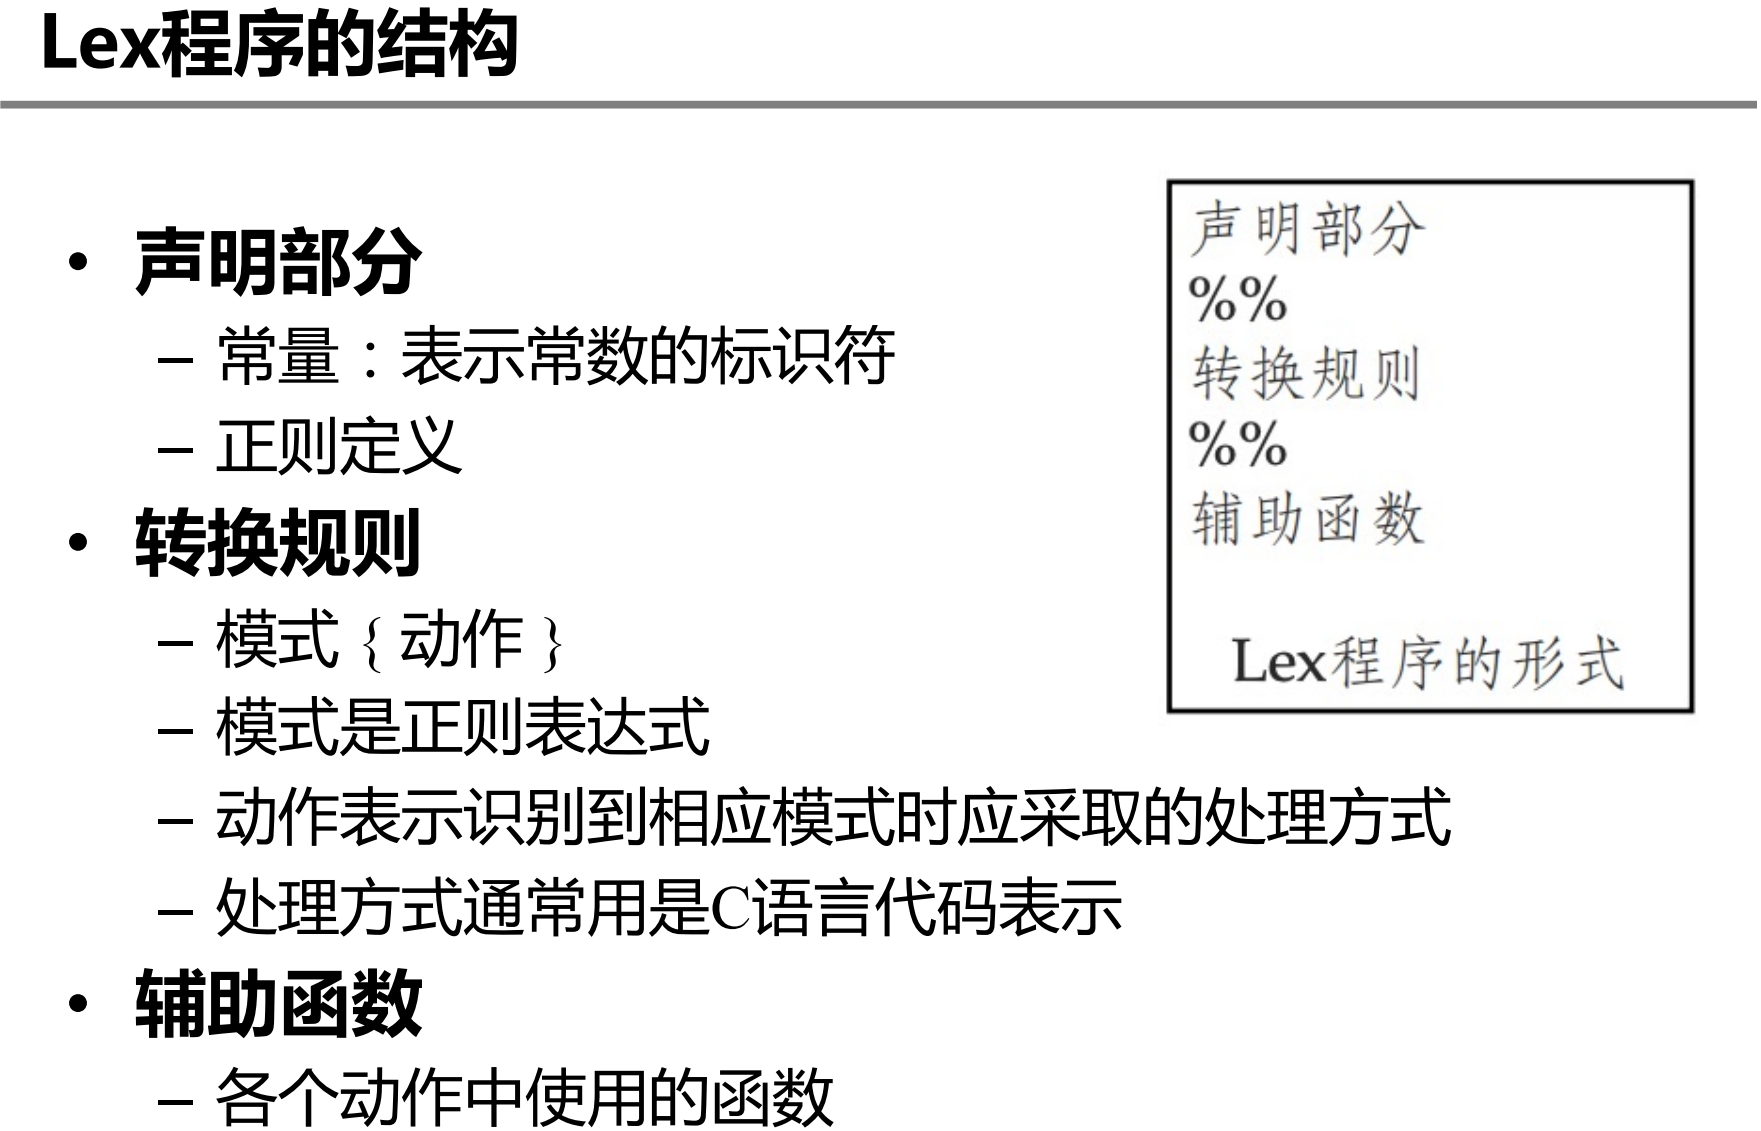
\includegraphics[width=0.4\linewidth]{figures/lex7.png}
    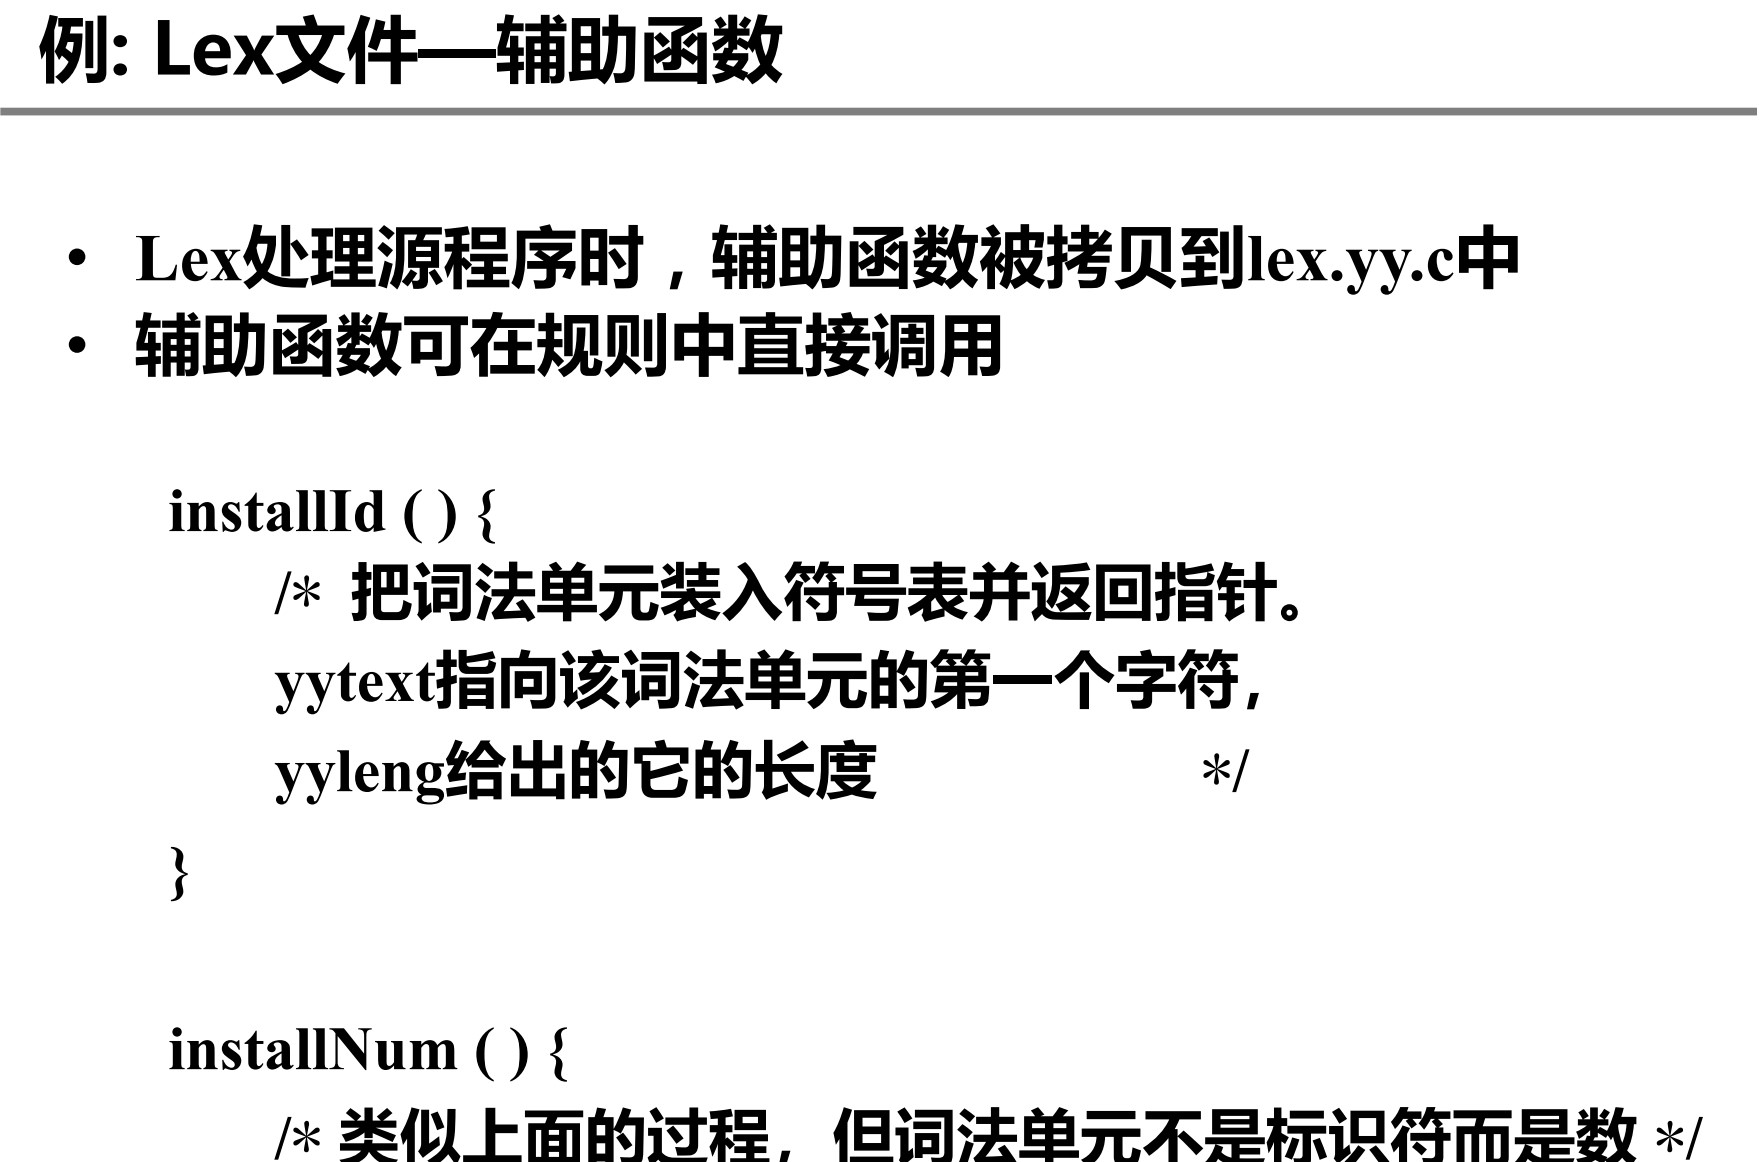
\includegraphics[width=0.4\linewidth]{figures/lex10.png}
    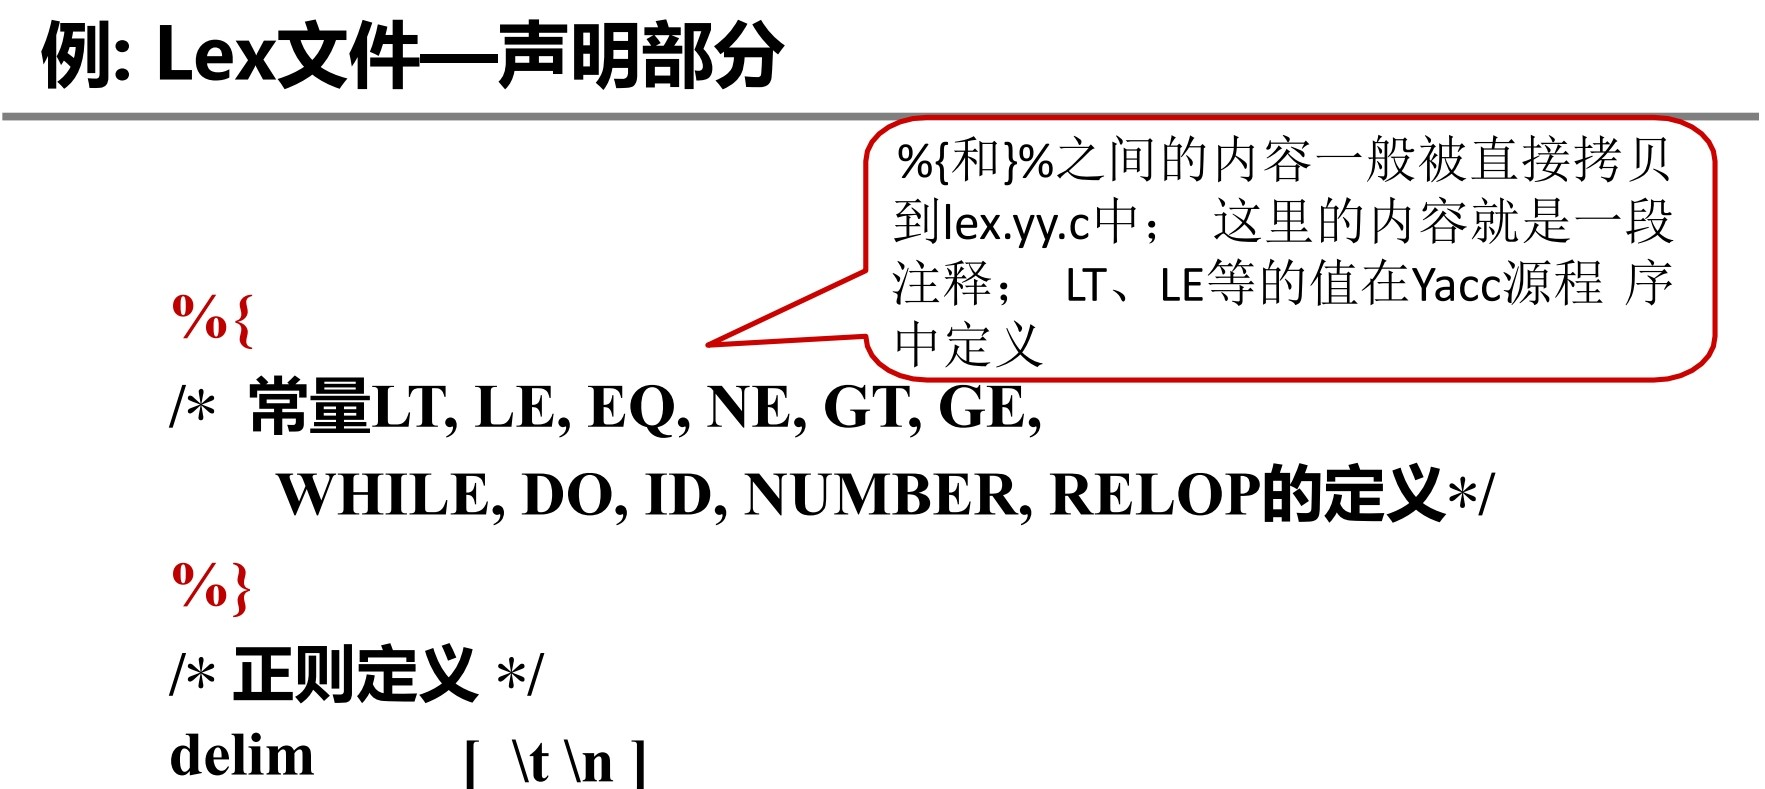
\includegraphics[width=0.4\linewidth]{figures/lex8.png}
    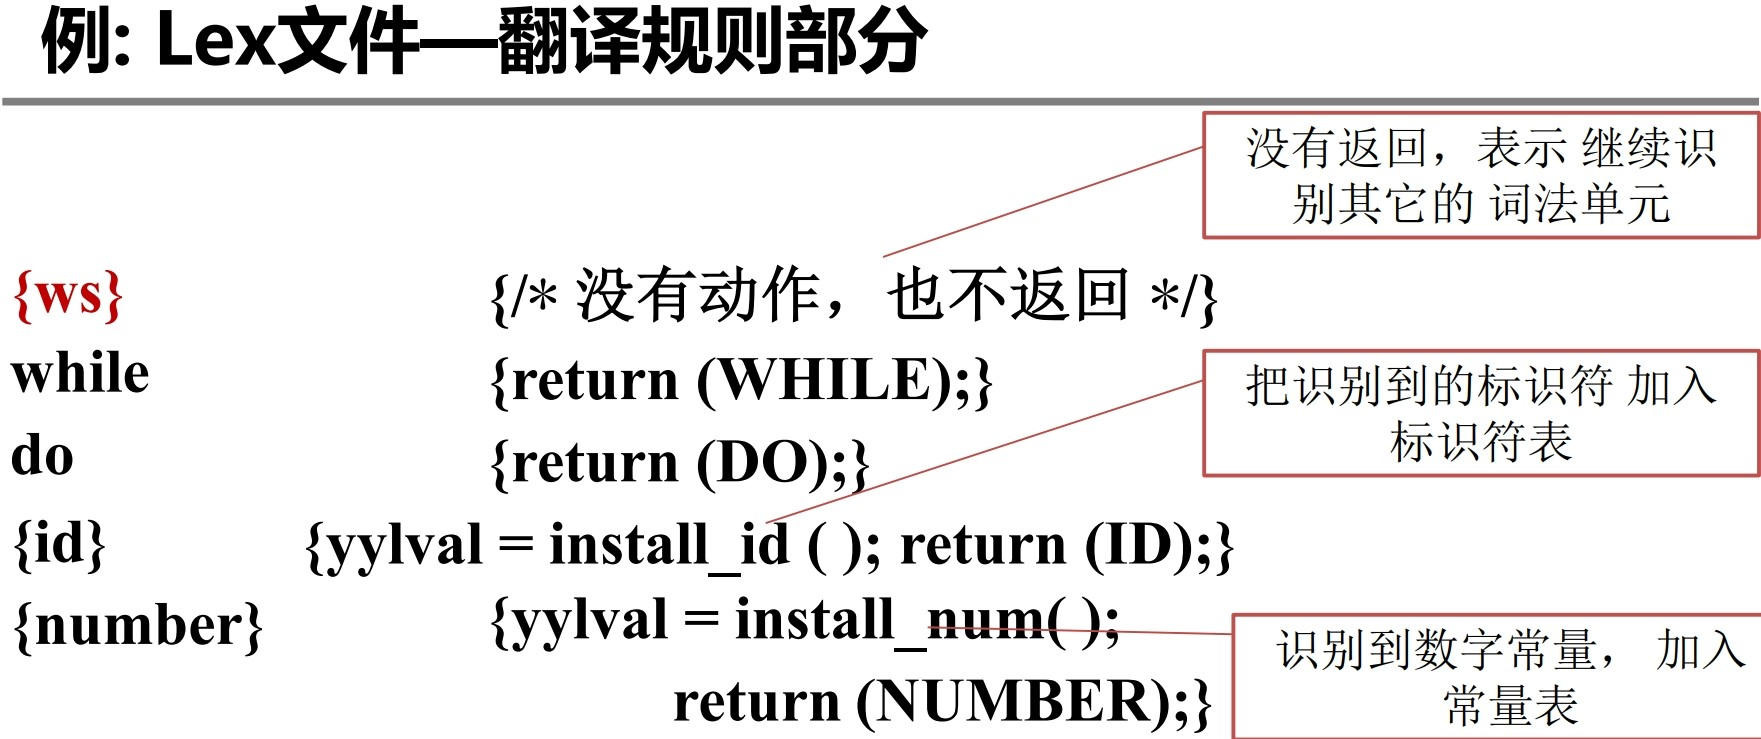
\includegraphics[width=0.4\linewidth]{figures/lex9.png}
\end{figure}
% ======================================================
% ======================================================
\section{Parsing}
\label{section:parsing}
% !TEX root = ./main.tex
% Parsing
% ======================================================
\par \noindent 推导:从文法的开始符号出发,逐步替换,直到推导出句子。
\par \noindent 归约:从句子出发,逐步替换,直到推导出文法的开始符号。
\par \noindent 最左推导: 每步代换最左边的非终结符(逆:最右规约),TD 分析:最左推导;
最右推导: 每步代换最右边的非终结符,(逆:最左规约),BU 分析:最左规约。
\par \noindent 句型(Sentential form) = 文法 G 下可能推导出的一个符号序列:可能包含终结符/非终结符/空。
\par \noindent 句子(Sentence) = 不含非终结符的句型(仅含终结符)。
\par \noindent 语言(Language) = 文法 G 可产生的所有句子的集合。
\par \noindent 上下文无关:$\alpha A \beta \rightarrow \alpha \gamma \beta$ 在推导过程中,符号串 $\gamma$ 仅依据对应产生式推导,
无需依赖上下文 $\alpha$,$\beta$。
\par \noindent 形式文法的分类:0 型文法(短语结构文法、递归可枚举语言)$\supset$ 1 型文法(上下文相关文法)
$\supset$ 2 型文法(上下文无关文法)$\supset$ 3 型文法(正则文法)。
\par \noindent 正则语言: 右线性文法(只有形如 $A \rightarrow a B$ 或 $A \rightarrow a$ 的产生式)/左线性文法产生的所有句子的集合。
\par \noindent 语法分析:不加限制的 CFG:$\mathcal{O}(n^3)$,LL(1) 文法:$\mathcal{O}(n)$,LR(1) 文法:$\mathcal{O}(n)$。
\par \noindent 设计编程语言文法:无二义性、(TD)无左递归、(TD)提左公因子。如果文法的某些句子存在不止一棵分析树,则该文法是二义的。
给定 CFG,判定有无二义性:不可判定问题。消除二义性:分层规定符号的优先级、结合性,确保只有一种最左推导。
\vspace{-10pt}
$$
\begin{array}{cc}
    \begin{array}{rl}
        E \rightarrow & E + E \\
        | & E \times E  \\
        | & (E)\ |\ id
    \end{array} &
    \begin{array}{l}
        E \rightarrow E + T\ |\ T \\
        T \rightarrow T \times F\ |\ F \\
        F \rightarrow (E)\ |\ id
    \end{array}
\end{array}
$$
\vspace{-15pt}
\par \noindent 改写:第一步/左式.(优先级)根据算符不同的优先级,为每一个算符引入新的非终结符,越接近开始符号的算符优先级越低
\par \noindent 改写:第二步/右式.(结合性)递归非终结符在终结符左边,运算就左结合,反之就右结合($+$ 与 $\times$)。
\par \noindent 允许回溯的递归下降分析(TD):按顺序尝试所有可能的产生式,出现问题就回溯。
% ======================================================
\subsection*{无回溯的自顶向下分析:LL(1) 分析}
\par \noindent 每次为最左边的非终结符号选择产生式时,向前看 1 个输入符号,预测要使用的产生式。
\par \noindent LL(1) 文法:任何产生式 $A \rightarrow \alpha\ |\ \beta$,其 $\alpha$ 和 $\beta$ 都满足:
1. $\first(\alpha) \cap \first(\beta) = \varnothing$;
2. 若 $\beta \Rightarrow^* \varepsilon$,那么 $\alpha \nRightarrow^* \varepsilon$,且 $\first(\alpha) \cap \follow(A) = \varnothing$。
LL(1) 文法是无二义的、无左递归的(不存在 $A \rightarrow^* A\alpha$)、无左公因子的(不存在 $A \rightarrow \alpha\beta\ |\ \alpha\gamma$)。

\par \noindent 如果非终结符 $X$ 可以推导出空串,则 $\nullable(x) = 1$:
(Base case)$X \rightarrow \varepsilon$;
(Inductive case) $X \rightarrow Y_1Y_2\cdots Y_n$,若 $Y_1, Y_2, \cdots, Y_n$ 都可推导出空串,则 $X$ 可推导出空串。

\par \noindent $\first(\alpha)$:可以从 $\alpha$ 推导出的串的首终结符集合:
(Base case)如果 $X$ 是终结符,$\first(X) = \{X\}$;
(Inductive case)如果 $X \rightarrow Y_1Y_2\cdots Y_n$,则 $\first(X) \cup = \first(Y_1)$;
如果 $Y_1$ 可推导出空串,则 $\first(X) = \first(X) \cup =  \first(Y_2)$,以此类推;
(推论)如果 $X \rightarrow a,\ a\in T$,则 $\first(X) \cup =\{a\}$。

\par \noindent $\follow(A)$:从起始符号 $S$ 推导出的串中,$A$ 后面可能出现的终结符集合:
(Base case)$\follow(S) = \{\}$;
(Inductive case)如果 $B \rightarrow \alpha A \beta$,则 $\follow(A) \cup = \first(\beta)$;
如果 $\beta$ 可推导出空串,则 $\follow(A) \cup = \follow(B)$。

\par \noindent LL(1) 预测分析表:表的每一行 $A$ 对应一个非终结符,表的每一列 $\alpha$ 对应某个终结符或输入结束符,
表中的项 $M(A, \alpha)$ 表示: 针对非终结符为 $A$,当下一个输入 Token 为 $\alpha$ 时,可选的产生式集,对于 LL(1) 文法,每个项最多只有一个产生式。

\begin{figure}[H]
    \centering
    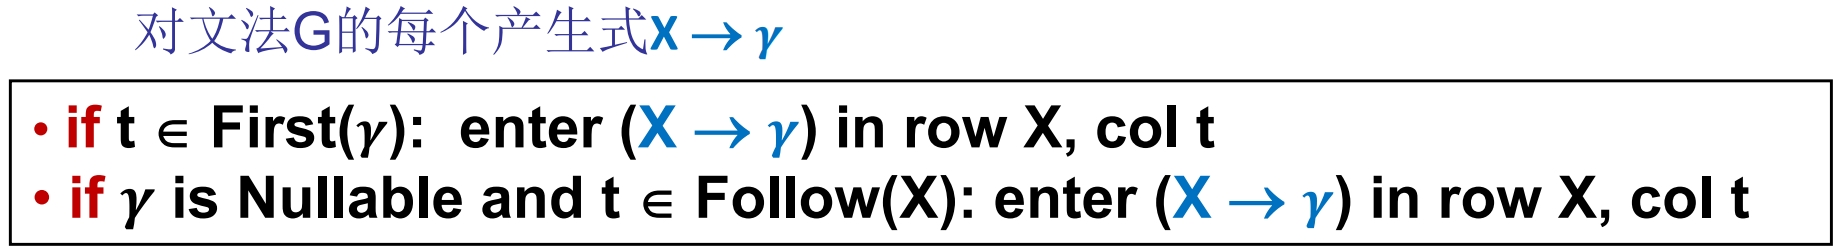
\includegraphics[width=\linewidth]{figures/LL1.png}
\end{figure}

\par \noindent 消除左递归和提左公因子:

\begin{figure}[H]
    \centering
    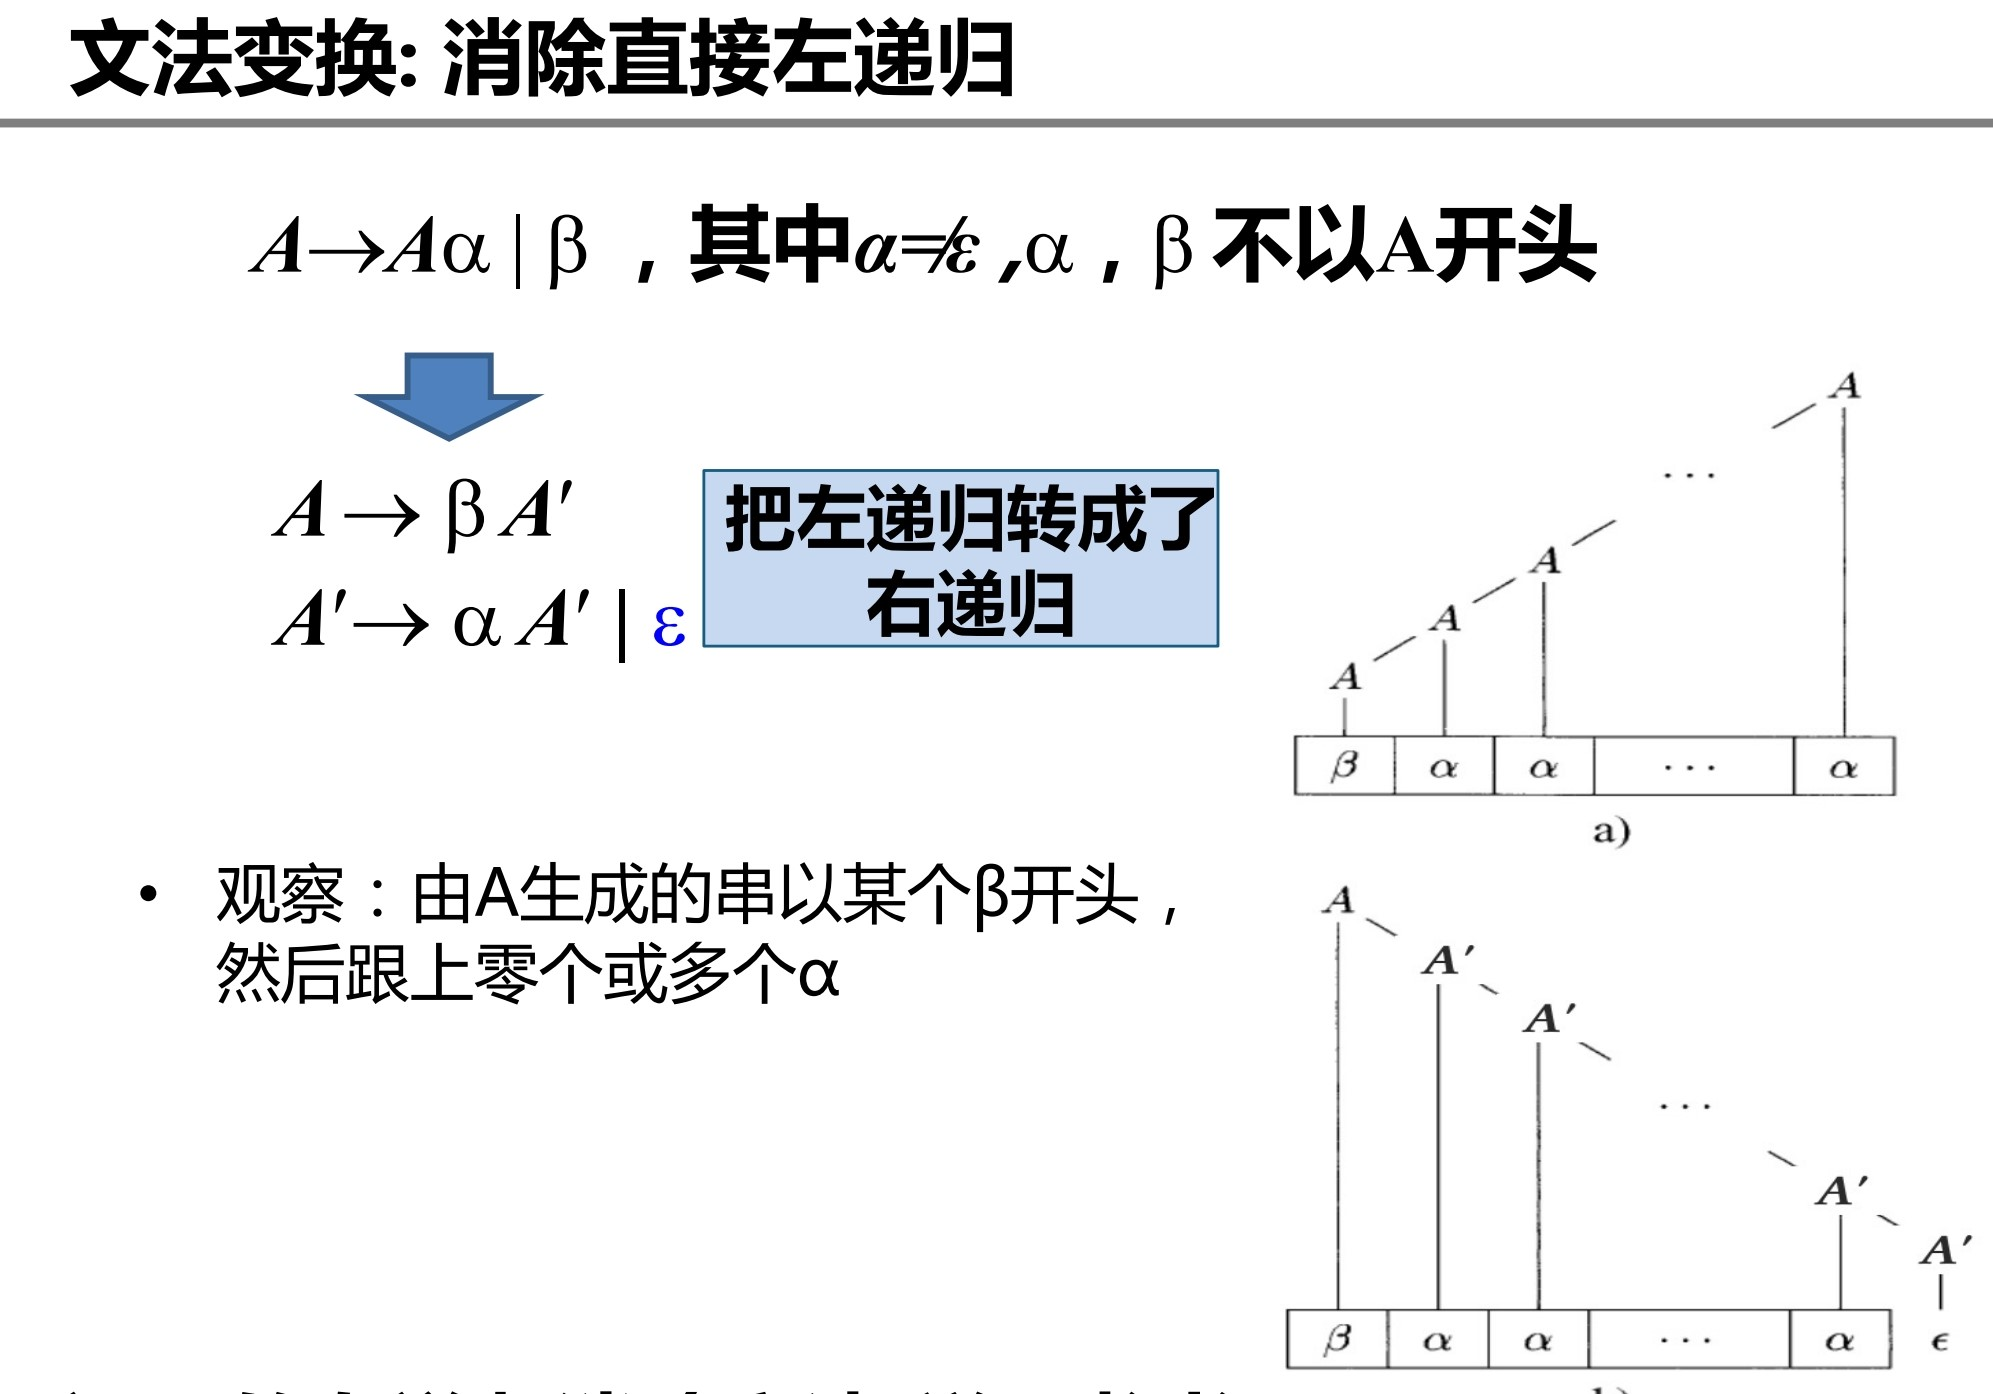
\includegraphics[width=0.48\linewidth]{figures/ll1gramma2.png}
    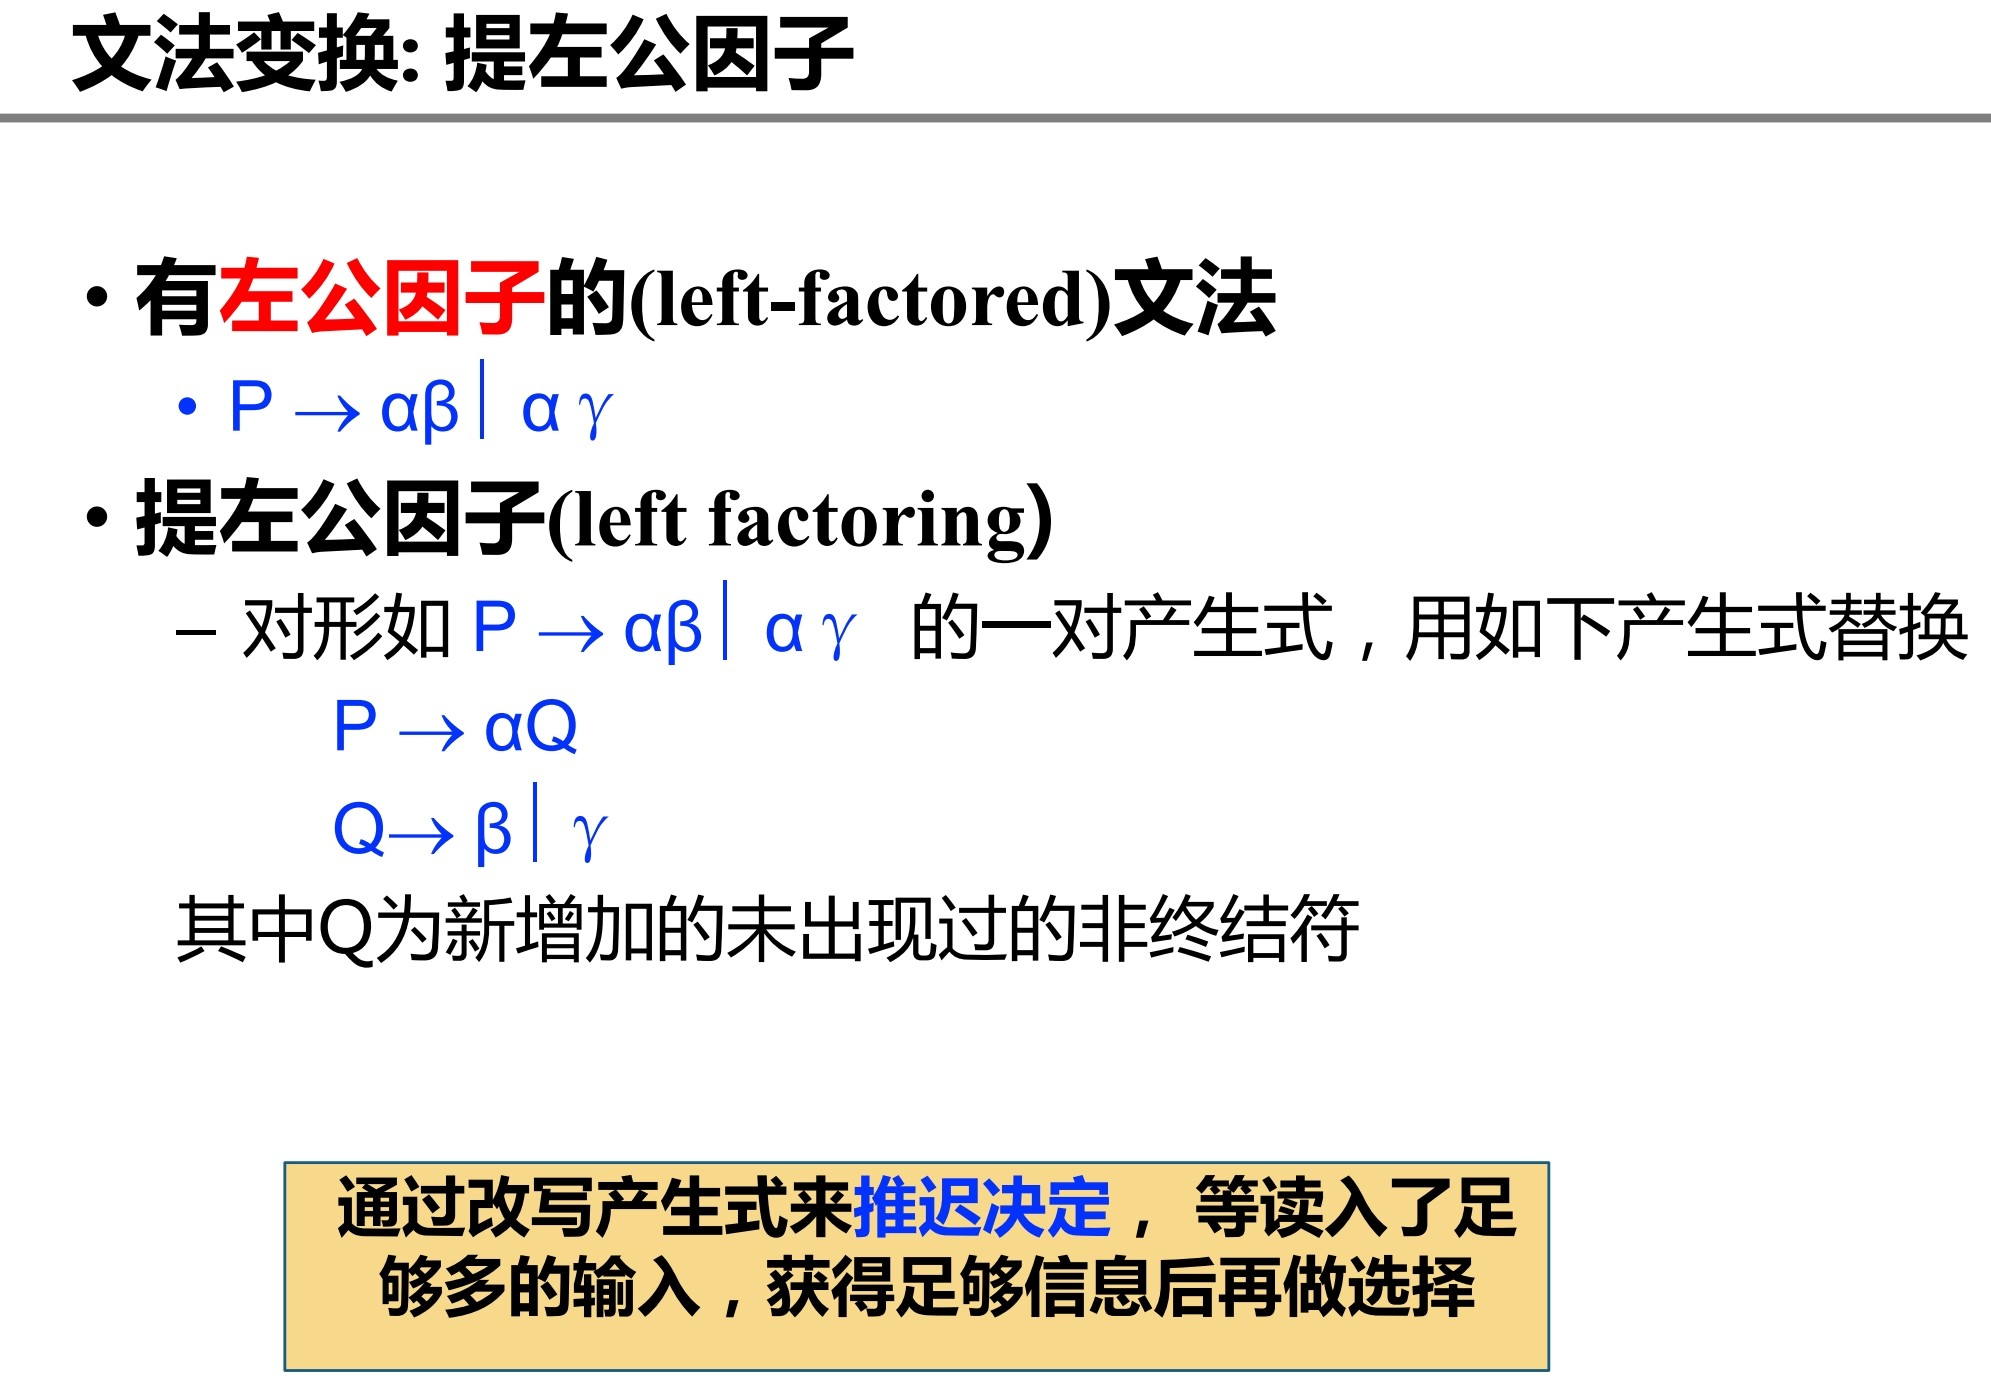
\includegraphics[width=0.48\linewidth]{figures/ll1gramma1.png}
\end{figure}

% LL(1) 错误恢复:不考
% ======================================================
\subsection*{自底向上分析:LR(0)、SLR、LR(1)、LALR 分析}

\par \noindent LR 分析: 最右推导的逆过程,限制了规约方式(类似 LL 中的最左推导)。
最右句型:最右推导过程中出现的句型, LR 分析的每一步都是最右句型,$\alpha | \beta$ 是最右句型

\par \noindent LR(0) DFA 构造、从 DFA 到语法分析表:

\begin{figure}[H]
    \centering
    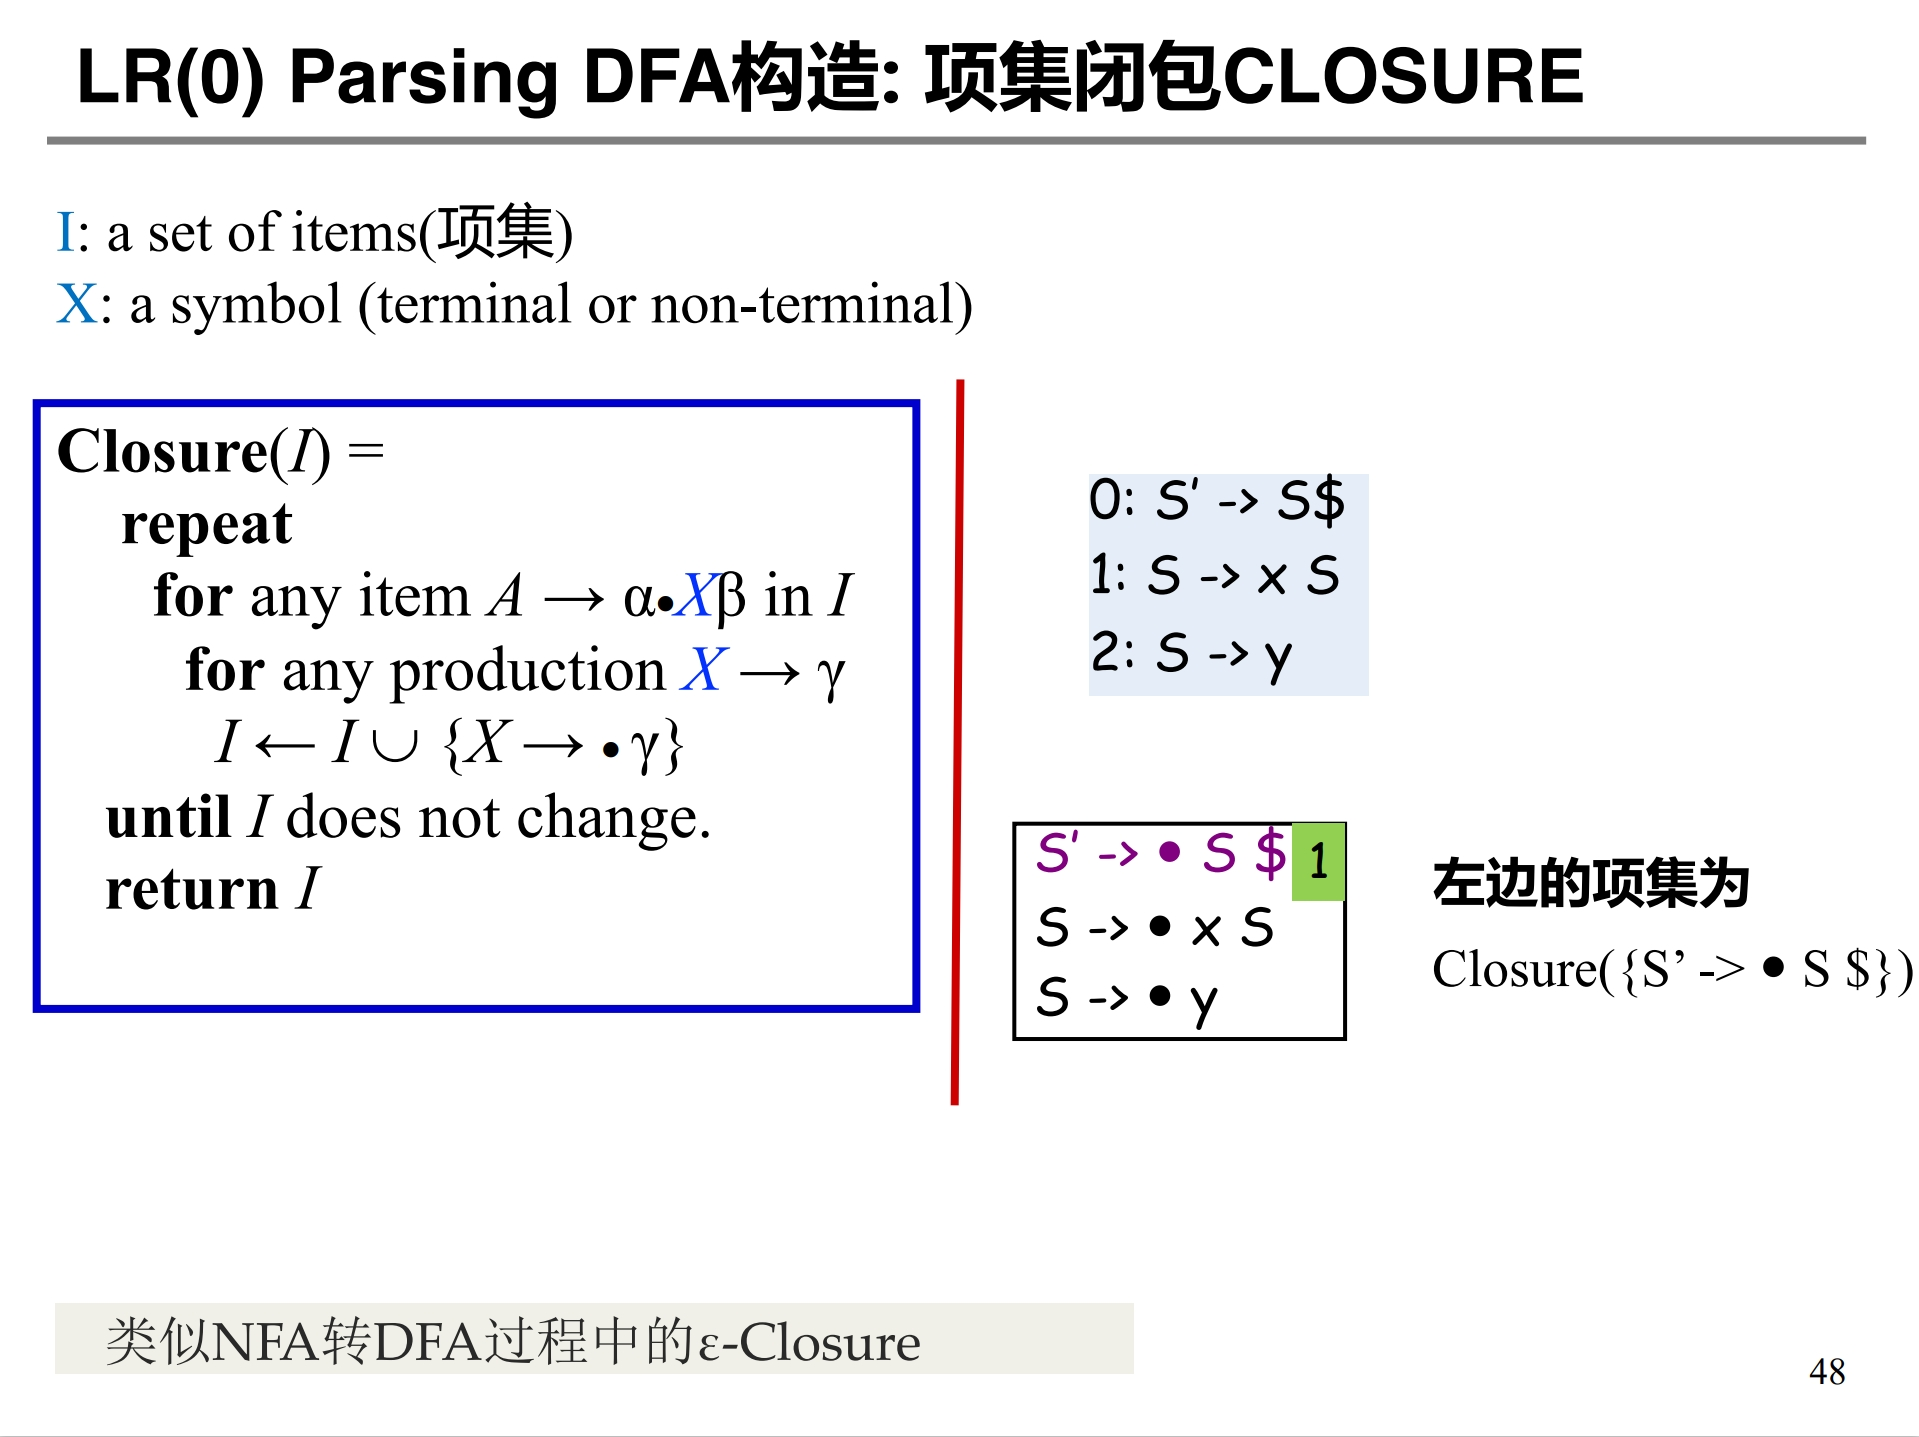
\includegraphics[width=0.48\linewidth]{figures/lr0-1.png}
    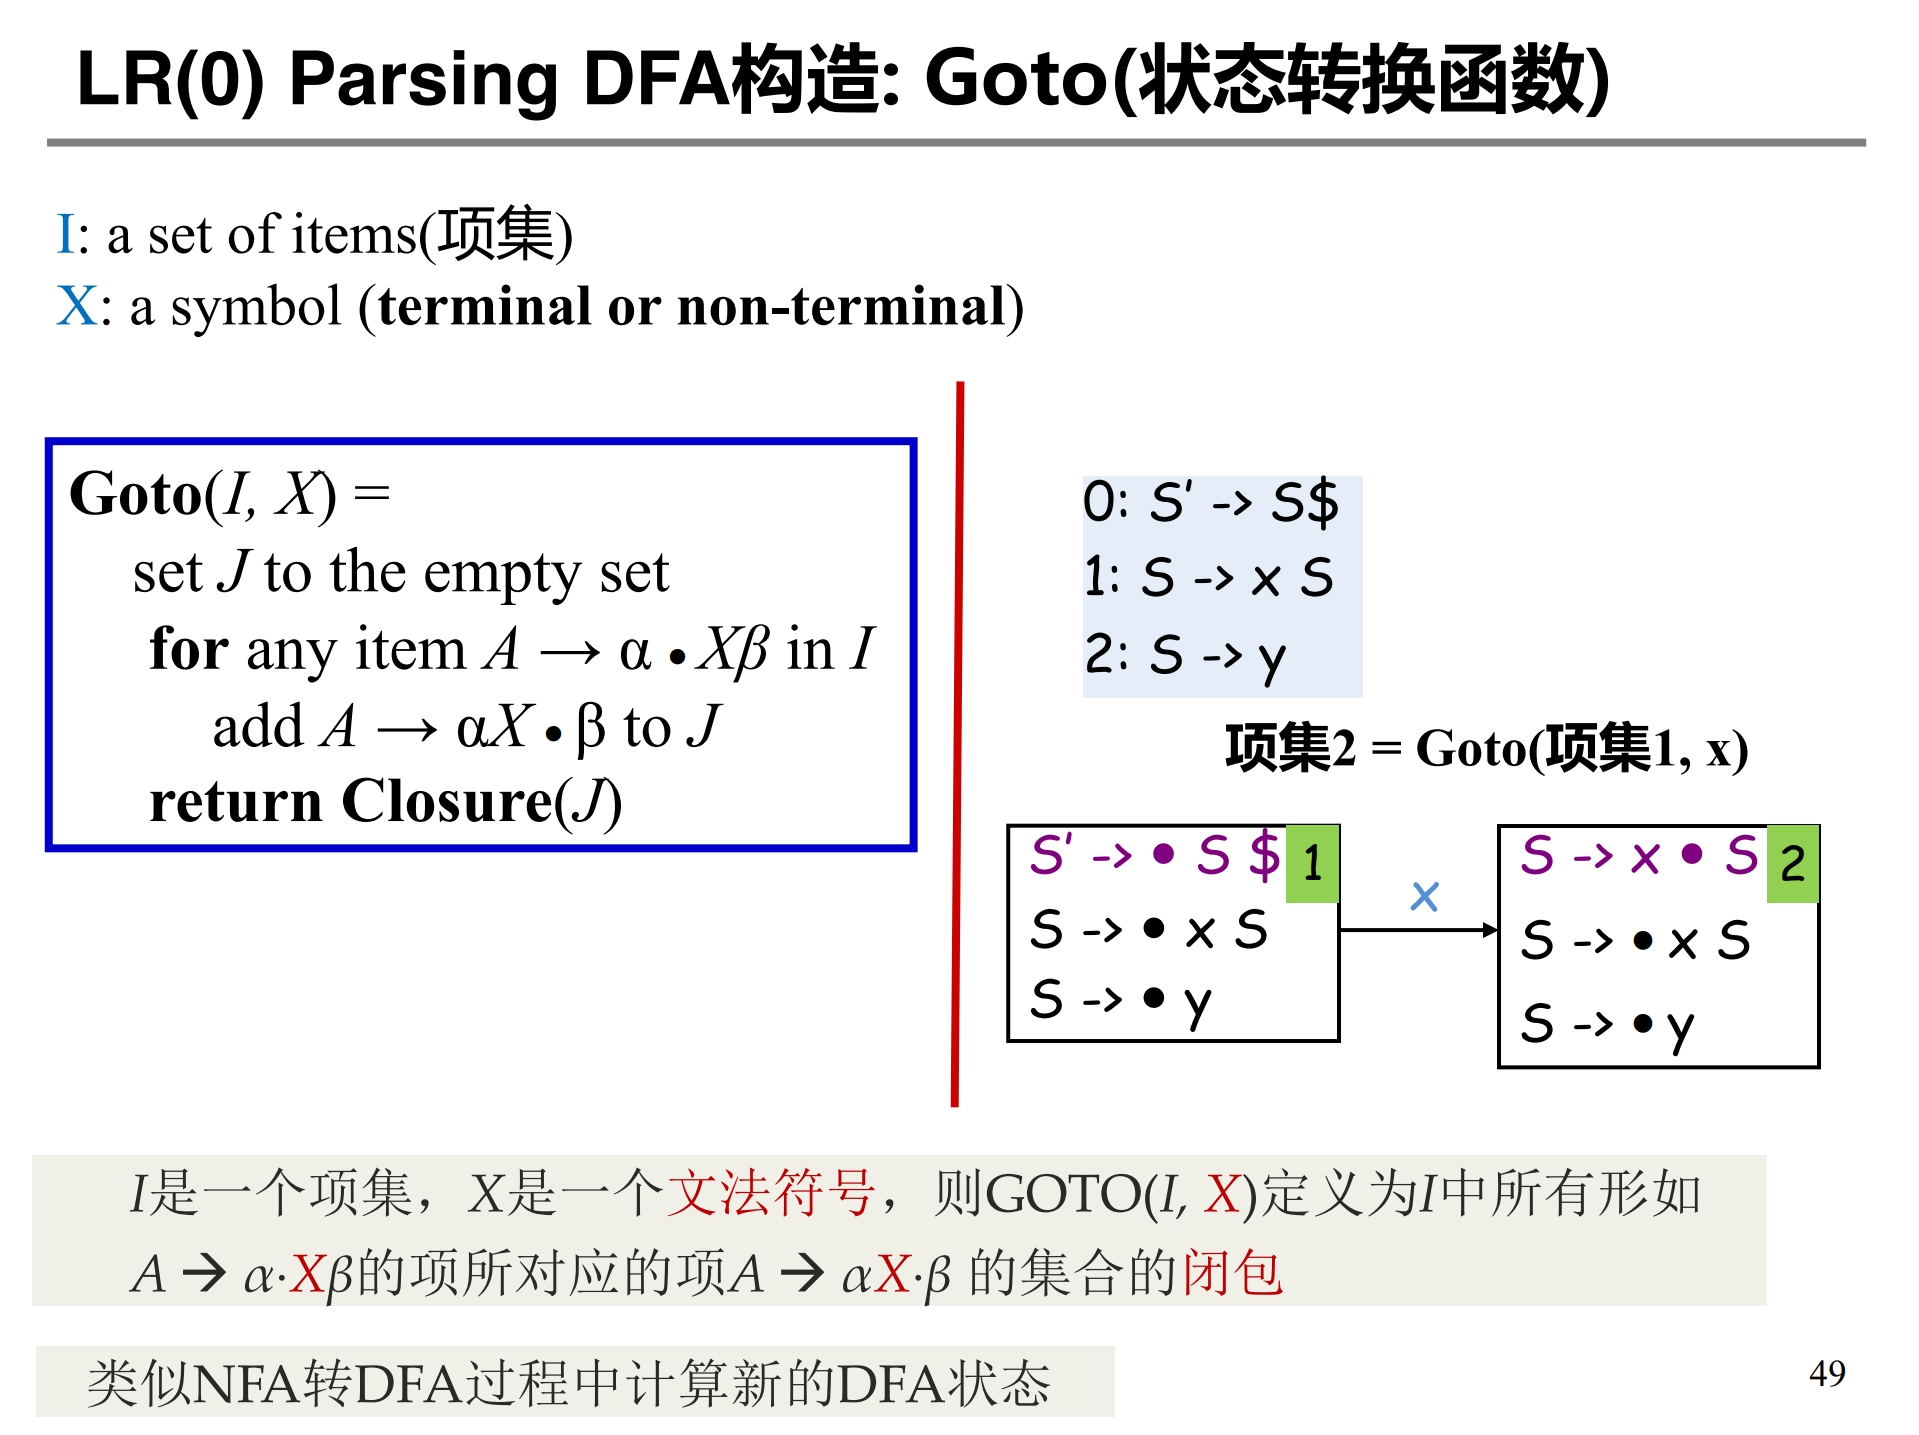
\includegraphics[width=0.48\linewidth]{figures/lr0-2.png}
\end{figure}

\begin{figure}[H]
    \centering
    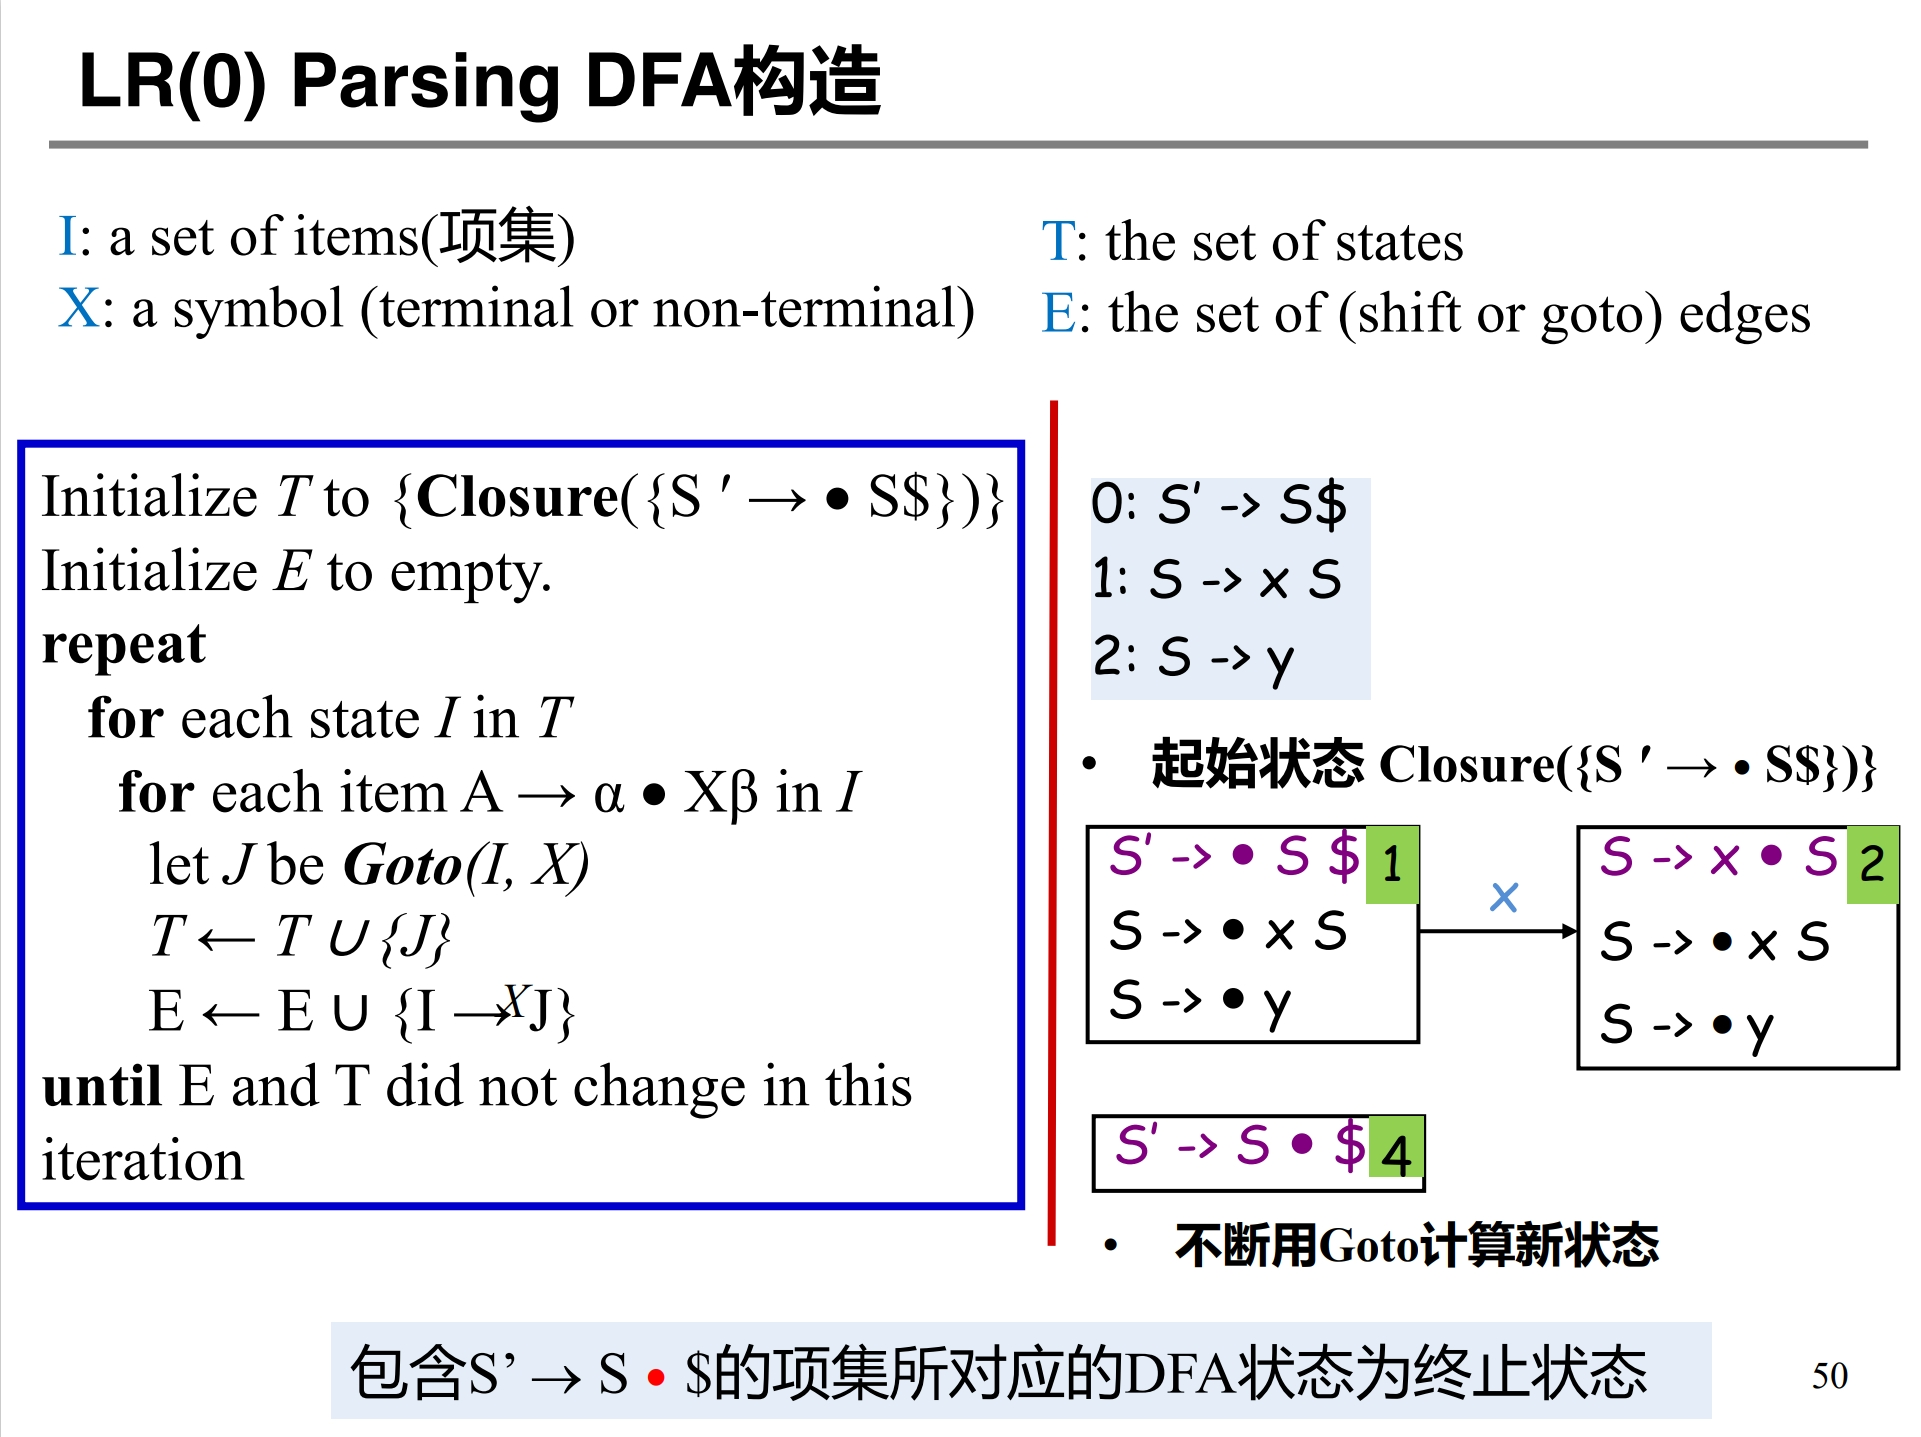
\includegraphics[width=0.48\linewidth]{figures/lr0-3.png}
    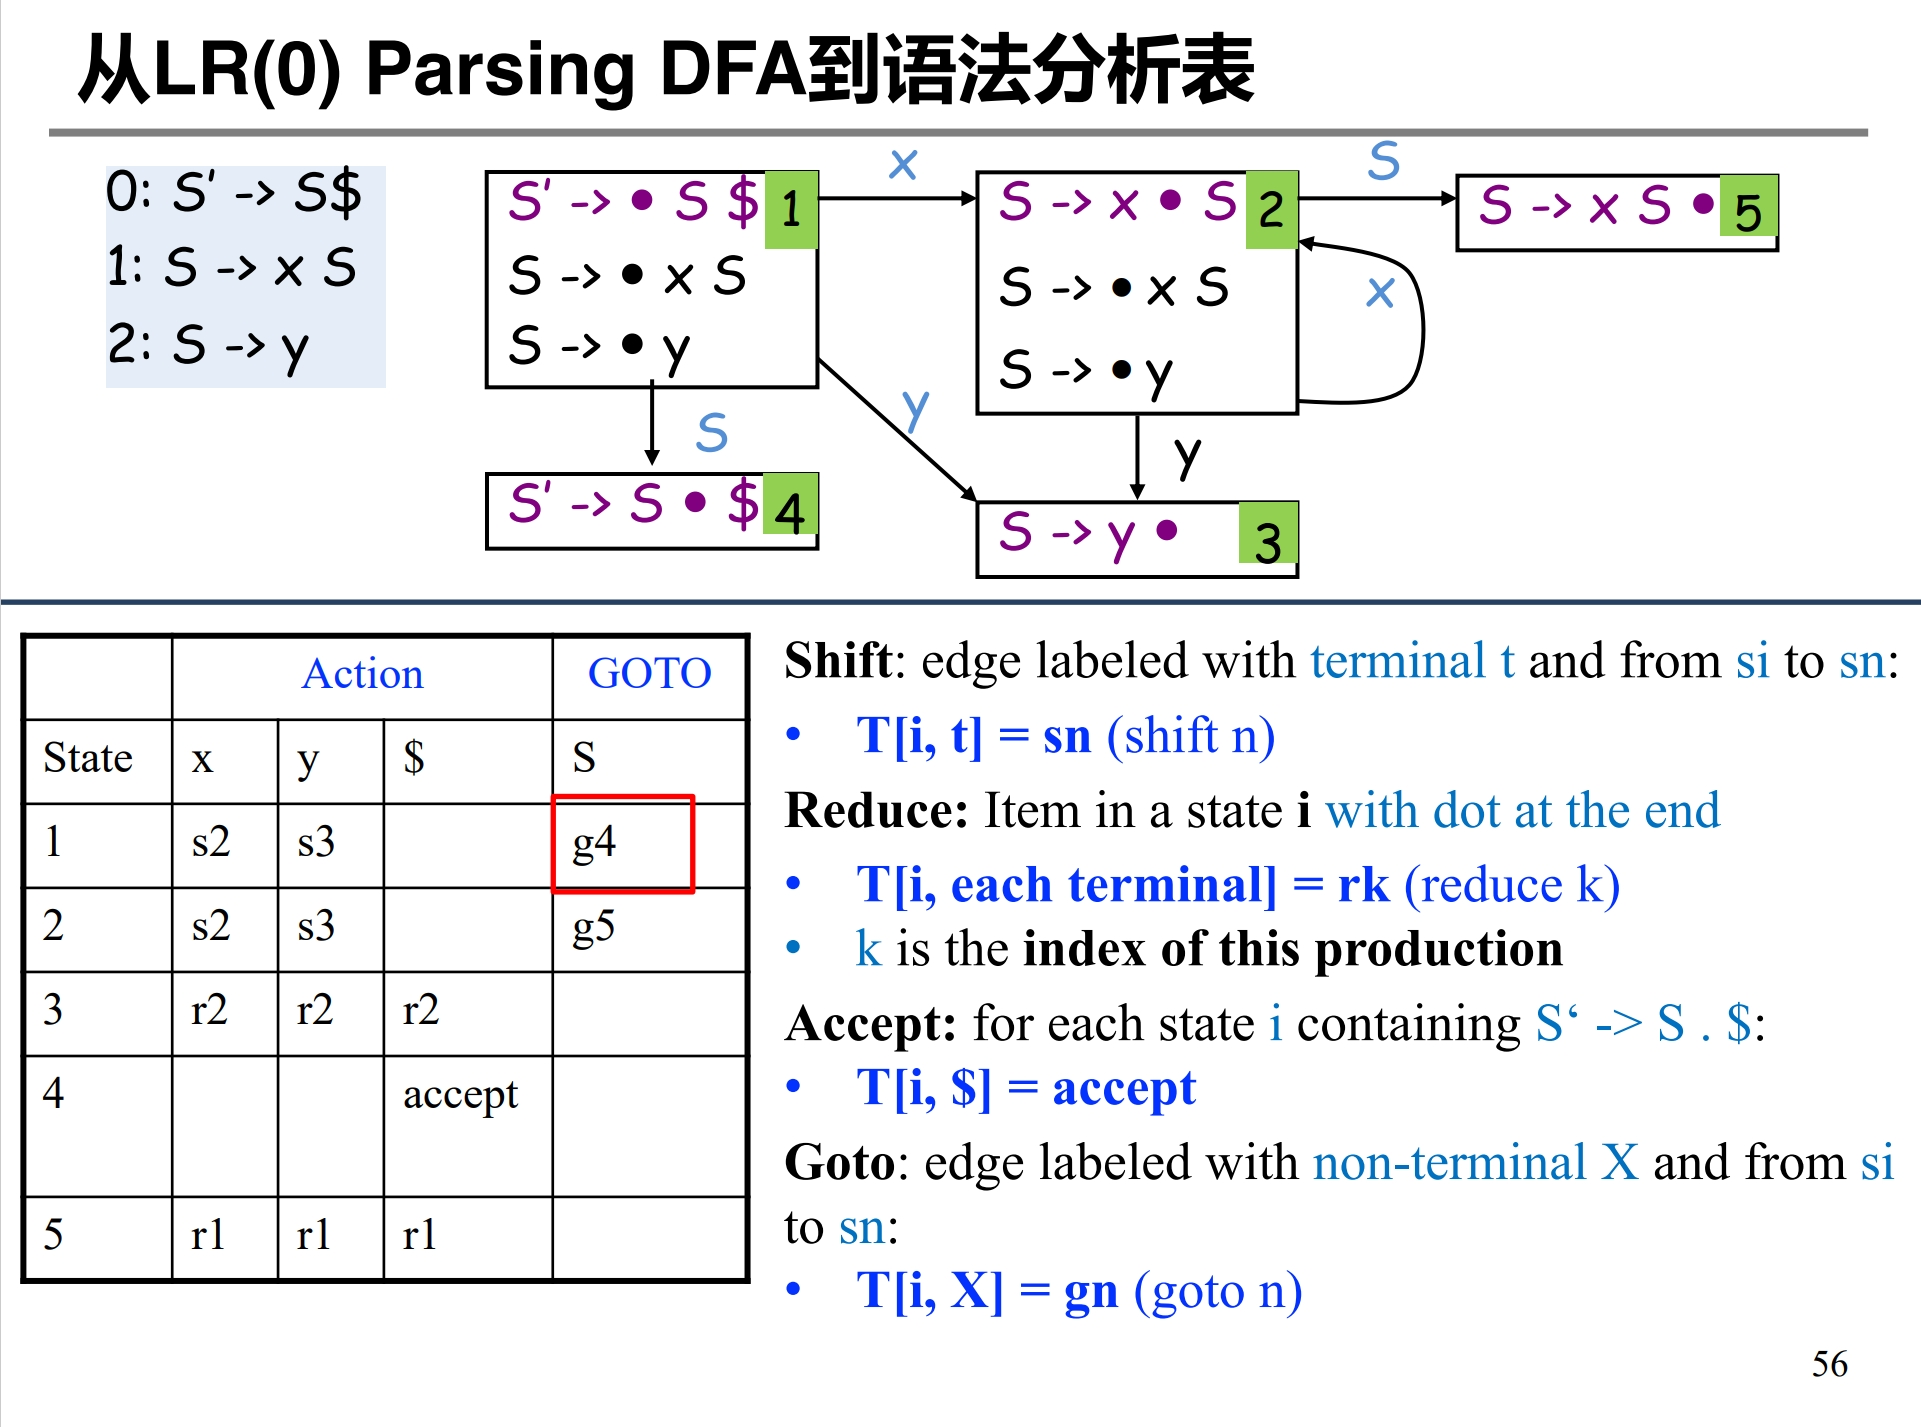
\includegraphics[width=0.48\linewidth]{figures/lr0-4.png}
\end{figure}

\par \noindent LR(0) 是否归约、选择哪个产生式规约仅由栈顶状态决定,对于每一个项 $X \rightarrow \alpha \bullet$ 盲目选择规约,可能导致 shift-reduce 冲突。

\par \noindent 使用更加严格的归约条件以降低冲突的可能性。规约条件更加严格 $\Rightarrow$ 语法分析表有更小的可能冲突 $\Rightarrow$ 识别更多文法。

\par \noindent SLR 分析:每步规约都应该满足 $t \in \follow(E)$,其中 $E$ 是用来归约的产生式的左部,$t$ 是下一个 token,在 LR(0) 分析表中划去不满足条件的规约项。
局限:如果 $\beta A x$ 不是任何最右句型的前缀,即使 $x$ 在某个句型中跟在 $A$ 之后,仍不应该按 $A \rightarrow \alpha$ 归约。可能会存在 shift-reduce 冲突。

\par \noindent LR(1) 分析:通过在项中添加 lookahead 符号以指导归约。

\par \noindent LR(1) 语法分析表的 Reduce Action 表项填写规则是:
对于规约 $A \rightarrow \alpha \beta \bullet,\ a$,填写到坐标为 (当前状态, $a$) 的单元格中。
其它表项填写规则以及 DFA 的生成规则与 LR(0)、SLR 一致。

\begin{figure}[H]
    \centering
    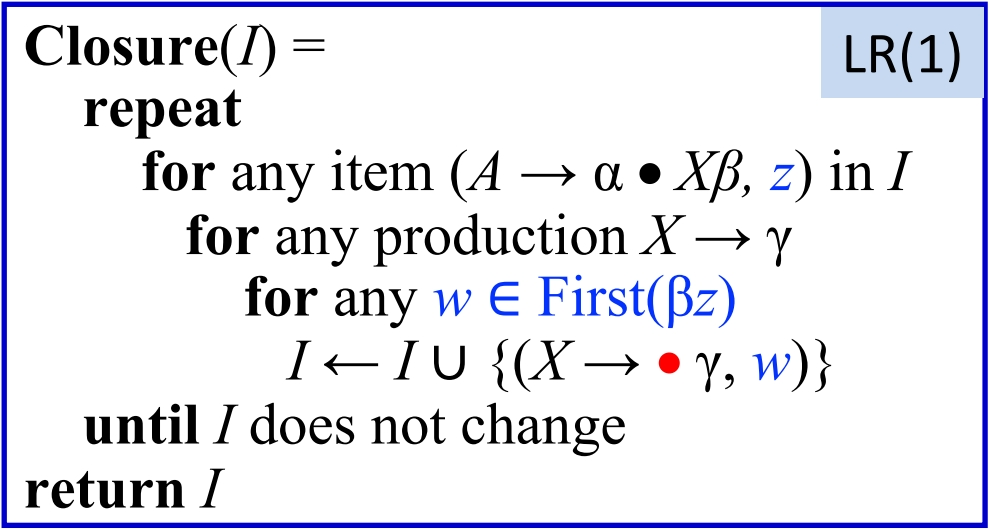
\includegraphics[width=0.48\linewidth]{figures/lr1-1.png}
    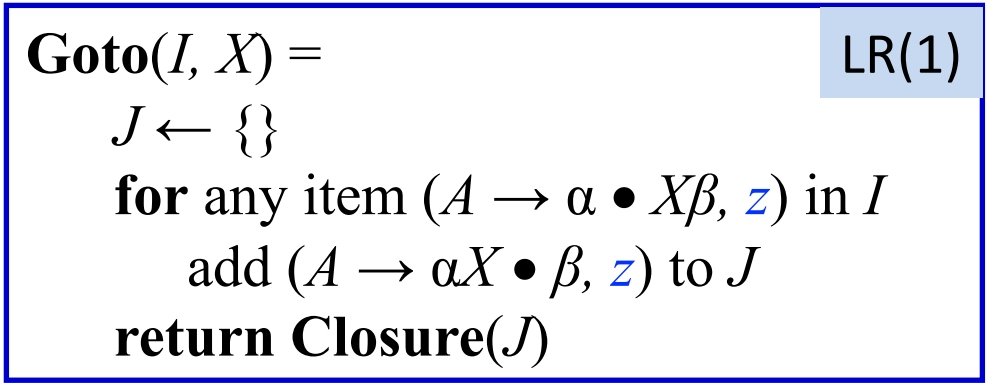
\includegraphics[width=0.48\linewidth]{figures/lr1-2.png}
\end{figure}

\par \noindent LALR 分析:介于 SLR(1) 和 LR(1) 之间,且分析表和 SLR 一样大。直到所有状态都有不同的核心(LR(1) 状态去掉所有项的 lookahead),重复下面的过程:
1. 选择两个具有相同核心的不同状态;2. 合并被选择的状态,创建一个包含所有原来状态中的项的新状态;3. 将所有指向原状态的边指向新状态,新状态指向所有原状态的后继状态。

\begin{figure}[H]
    \centering
    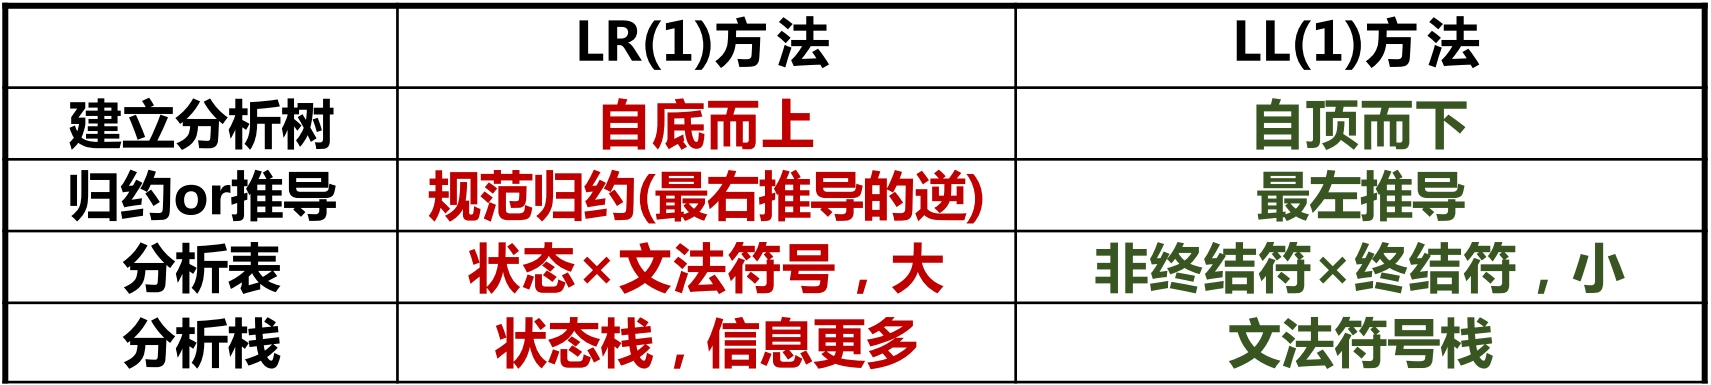
\includegraphics[width=\linewidth]{figures/parsing.png}
\end{figure}

% 自底向上分析中的错误恢复:不考
% ======================================================
\subsection*{YACC}
\par \noindent 基于 LALR(1),用 BNF 形式书写。GNU 版:Bison。
\par \noindent YACC 程序结构:声明区(放置 C 声明和对词法单元的声明)、翻译规则区(指明产生式及相关的语义动作)、
辅助性 C 语言例程区(被直接拷贝到生成的 C 语言源程序中。可在语义动作中调用。包括 \texttt{yylex()},这个函数返回词法单元,可以由 Lex 生成),
互相之间用 \texttt{\%\%} 分隔。
\par \noindent YACC/Bison 语义动作和文法的对应关系:在使用规则执行规约操作后,将执行\texttt{\{}语义动作\texttt{\}}指定的操作。
翻译规则例:\texttt{exp: exp '+' term \{\$\$ = \$1 + \$3;\}},
其中\texttt{\$\$} 表示和产生式头相关的属性值,\texttt{\$i} 表示产生式体中第i个文法符号的属性值。
\par \noindent 消除二义性: 为算符指定优先级与结合律。冲突解决:归约-归约冲突 $\rightarrow$ 选择 Yacc 说明中先出现的产生式;
移进-归约冲突 $\rightarrow$ 移近优先。
% ======================================================
\section{Abstract Syntax}
\label{section:abstract-syntax}
% !TEX root = ./main.tex
% Abstract Syntax
% ======================================================
\par \noindent 属性文法 = 上下文无关文法 + 属性 + 属性计算规则。
属性: 描述文法符号的语义特征,如变量的类型、值等(例: 非终结符 E 的属性 E.val = 表达式的值);
属性计算规则(语义规则): 与产生式相关联、反映文法符号属性之间关系的规则(例: 如何计算E.val),
仅表明属性间抽象关系,不涉及具体实现细节,如计算次序等。
应用:程序分析表达式的类型、值、执行代价;抽象语法树生成、中间代码甚至汇编生成。
可通过 Parser 生成器支持的语义动作(Semanticaction)实现计算,并应用于抽象语法树生成等场景。

\par \noindent 抽象语法树:不依赖于具体语法细节的树形结构,比解析树简洁,没有无意义的终结符节点。

\par \noindent 关于错误位置:parser 维护一个位置堆栈以及语义值堆栈,使每个符号的位置可供语义操作使用(Bison);
定义一个非终结符 \texttt{pos},其语义值是源位置(行号,或行号和行内位置)(Yacc)。
% ======================================================
\section{Semantic Analysis}
\label{section:semantic-analysis}
% !TEX root = ./main.tex
% Semantic Analysis
% ======================================================
\par \noindent 语义分析:引用的维度是否与声明匹配、数组访问是否越界、变量应该存储在哪里\dots(这些问题取决于值而不是语法)
\par \noindent 狭义语义分析:通过 AST 确定程序的一些静态属性,例如名称的范围和可见性(每个变量在使用前都已声明)、
变量、函数和表达式的类型(每个表达式都有适当的类型、函数调用符合定义)。

\par \noindent 符号表:环境的实现;环境:绑定的集合;绑定:$\text{Name/Symbol} \mapsto \text{Meaning/Attribute}$;属性:类型、值、函数签名等。
环境:$\sigma_1 = \sigma_0 + \{a \mapsto \text{int}, b \mapsto \text{int}, c \mapsto \text{int}\}$,
$\sigma_2 = \sigma_1 + \{a \mapsto \text{str}\}$,等式右侧的符号表将覆盖左侧的符号表(现在 $a \mapsto \text{str}$)。

\par \noindent 符号表的实现:Imperative(例:bucket list / hash table)使用哈希查找对应标识符在表中的位置(bucket),
插入新环境时,在对应标识符 bucket 顶部插入新绑定,恢复环境时,从对应 bucket pop 绑定。
Functional(例:persistent BST)使用可持久化维护数据结构的历史,退出 scope 时回到相应的历史状态,
插入新环境时只复制标识符在树中的所有祖先(避免完整拷贝所有旧版本)。
% ======================================================
\section{Activation Record}
\label{section:activation-record}
% !TEX root = ./main.tex
% Activation Record
% ======================================================
\par \noindent 活动记录 = 栈帧。
函数调用:1. Push arguments;2. Push return address;3. Save caller-save registers;4. Jump to called function。
被调用函数:1. \texttt{push rbp},\texttt{mov rbp, rsp};2. Save callee-save registers;3. Allocate space for local variables。
函数返回:1. Restore callee-save registers;2.\texttt{mov rsp rbp},\texttt{pop rbp};3. Pop return address;4. Jump back to caller。

\par \noindent 块结构:在允许嵌套函数声明的语言(如 Tiger)中,内部函数可以使用在外部函数中声明的变量,实现方式:

\par \noindent Static link:每次调用函数 g 时,可以将指向静态包围 g 的函数的栈帧的指针在栈中传递给 g(这个指针就是 static link)。
每个函数都带有其嵌套深度的注释,当深度为 $n$ 的函数访问在深度为 $m$ 的函数中的变量时,向上爬 $n-m$ 个链接以访问适当的活动记录。
优点:参数传递时额外开销小;缺点:访问非局部变量时需要向上爬静态链接链,每个变量访问需要一条链,链的长度等于变量声明函数和使用函数的嵌套深度之差。

\par \noindent Lambda Lifting:当 f 调用 g 时,f 中实际访问的每个变量都作为额外参数传递给 g。

\par \noindent Display:可以维护一个全局数组(称为 display),display[i] = 指向最近进入的、其静态嵌套深度为 i 的过程的栈帧的指针。

\begin{figure}[H]
    \centering
    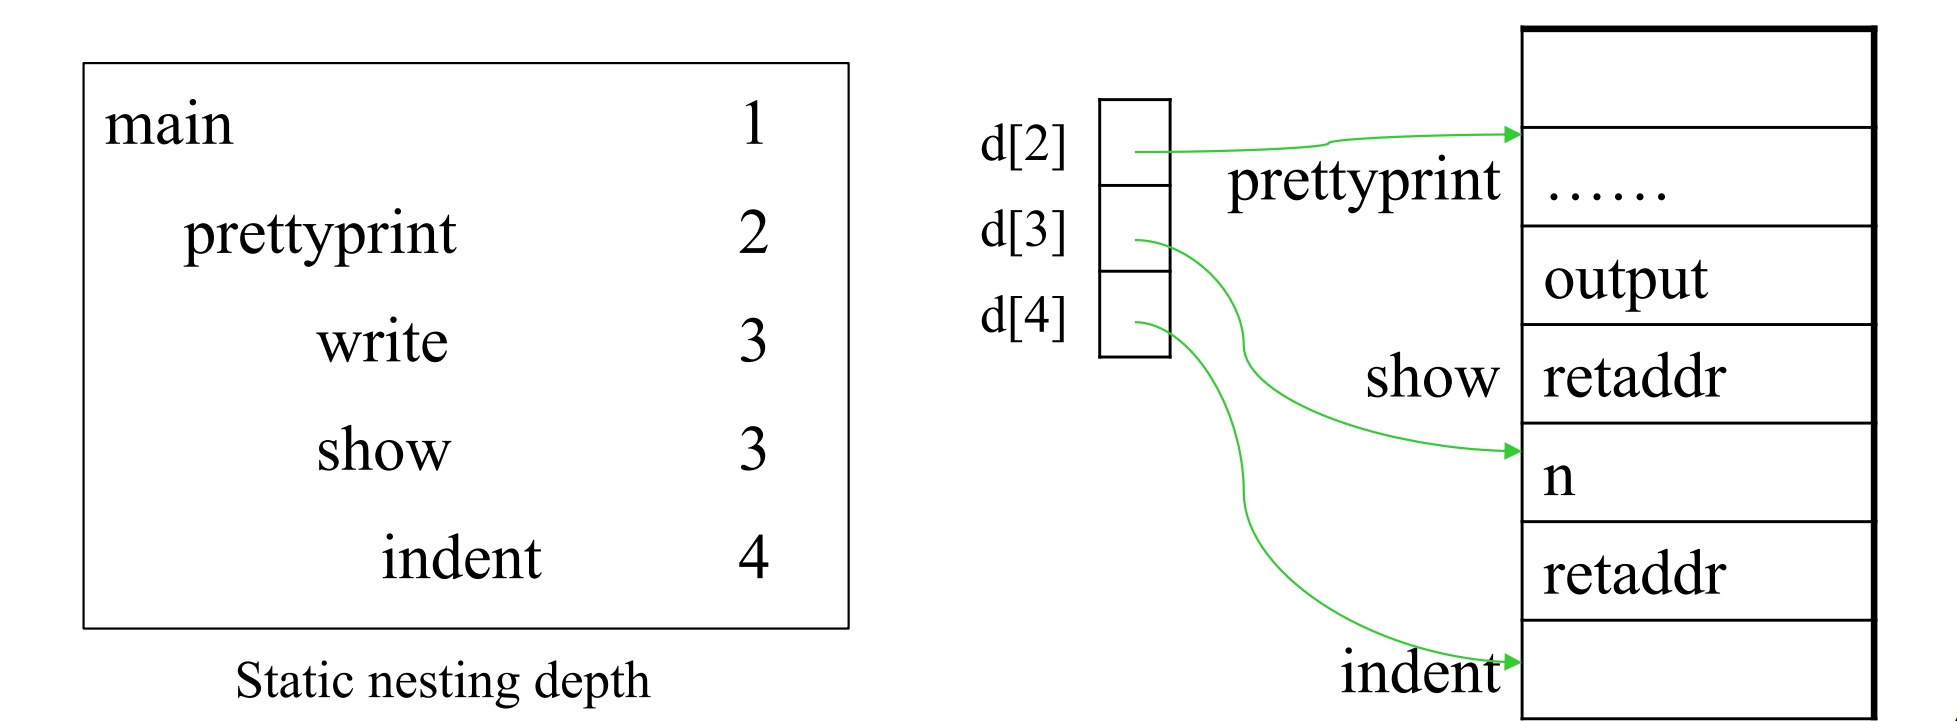
\includegraphics[width=0.8\linewidth]{figures/ar1.png}
\end{figure}

\begin{figure}[H]
    \centering
    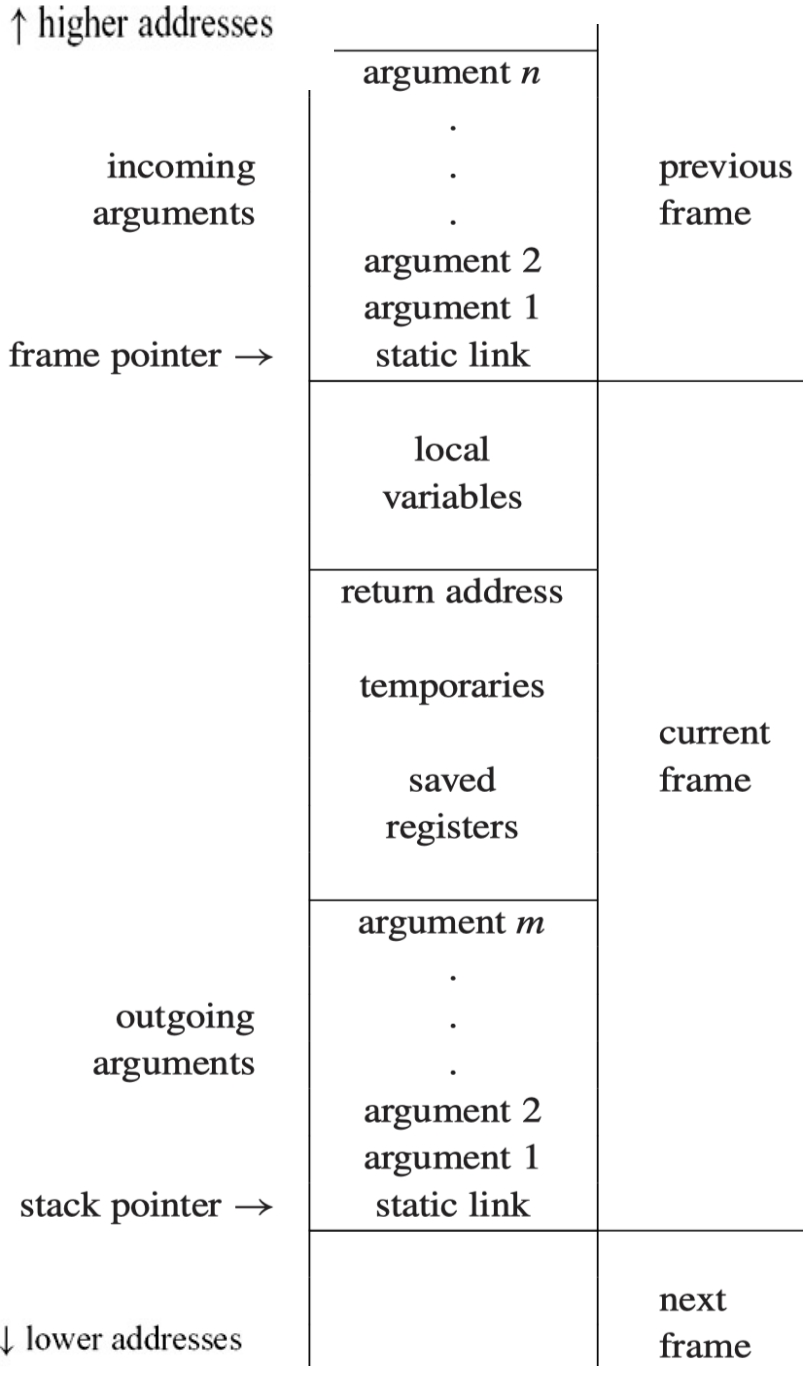
\includegraphics[angle=90, width=0.8\linewidth]{figures/ar2.png}
\end{figure}
% ======================================================
\section{Translating into Intermediate Code}
\label{section:ir}
% !TEX root = ./main.tex
% Translating into Intermediate Code
% ======================================================

\begin{figure}[H]
    \centering
    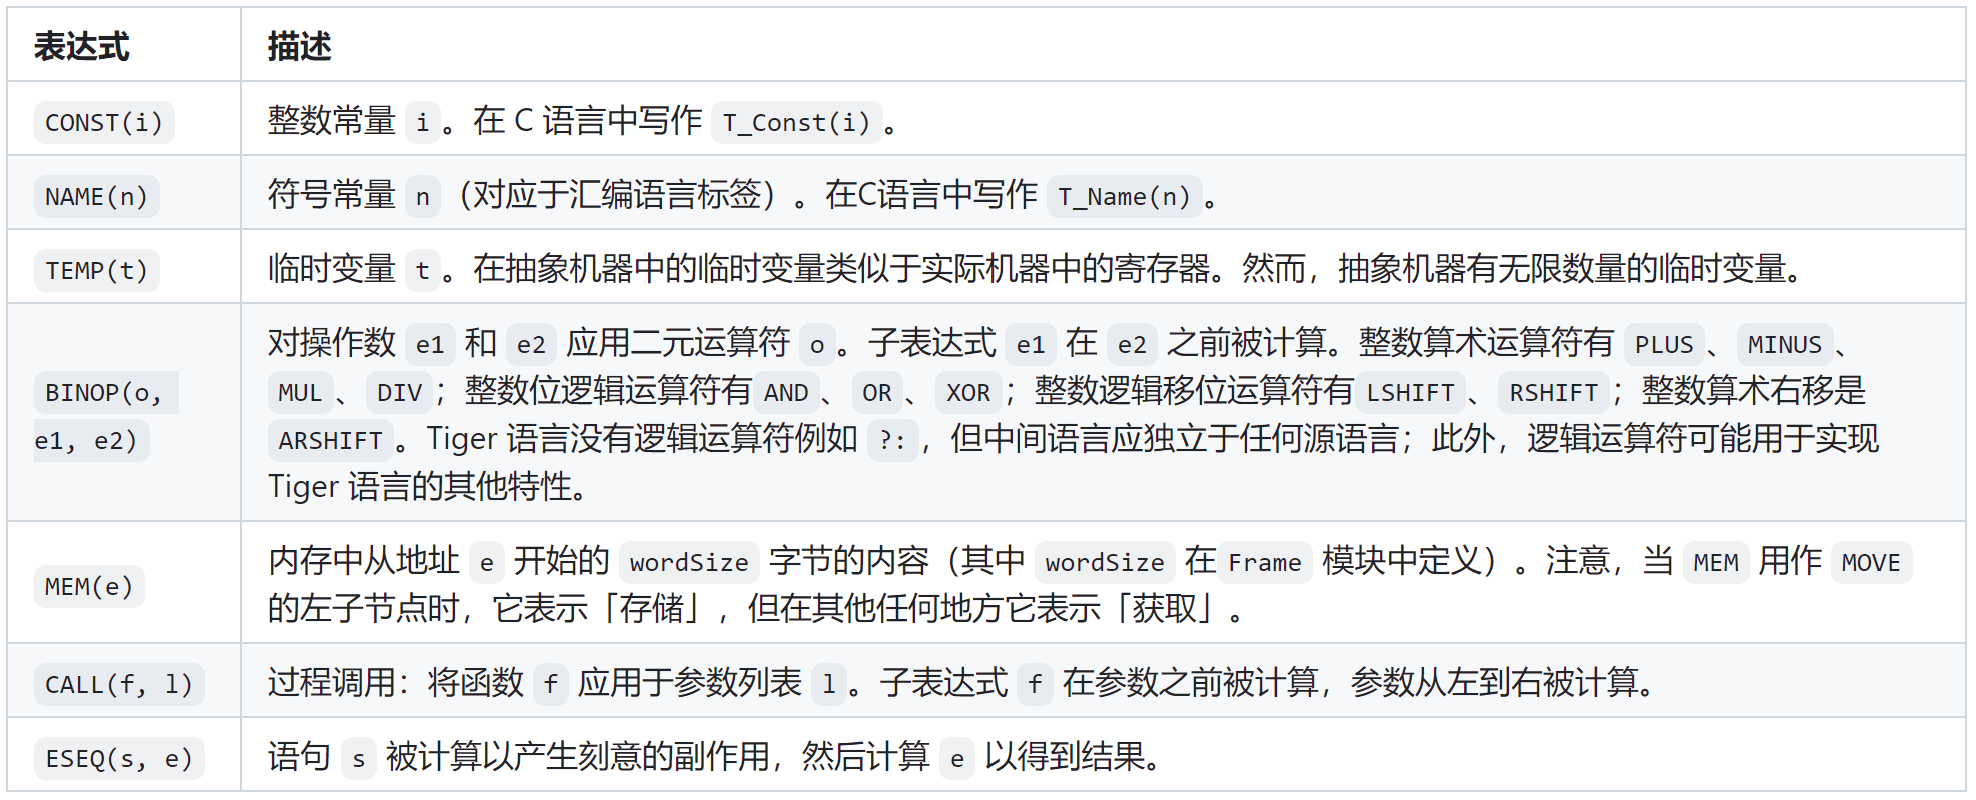
\includegraphics[width=\linewidth]{figures/ir2.png}
\end{figure}

\begin{figure}[H]
    \centering
    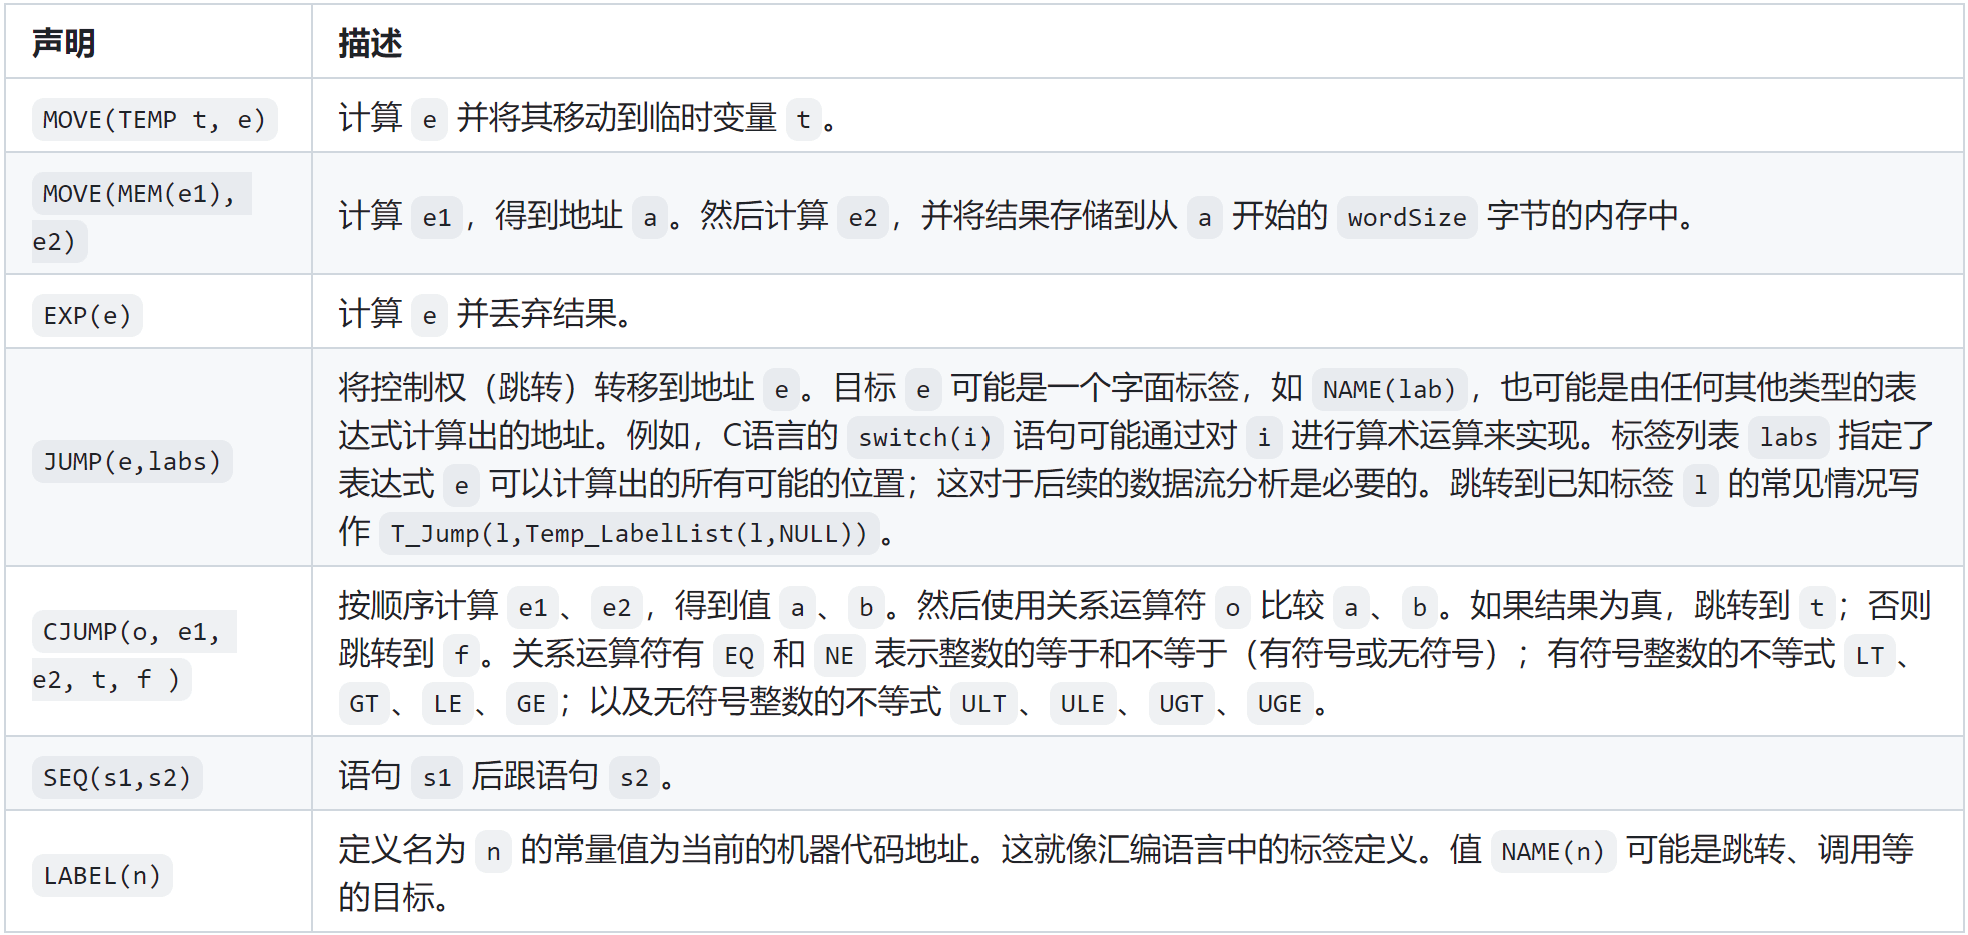
\includegraphics[width=\linewidth]{figures/ir1.png}
\end{figure}

\par \noindent 函数调用:\texttt{CALL(NAME lf , [sl, e1, e2, . . . , en])},其中 \texttt{lf} 是函数标签,
\texttt{sl} 是 static link,\texttt{e1, e2, . . . , en} 是参数。函数被翻译为 prologue、body 和 epilogue 三部分,
prologue = 
1. 声明一个函数开始的伪指令;
2. 函数名 label 的定义;
3. 调整栈指针、分配新的栈帧;
4. 将逃逸(escaping)参数保存至栈帧、将非逃逸参数传送到新临时寄存器;
5. 保存此函数用到的 callee-save 寄存器(包括返回地址寄存器)。
body = 函数体。
epilogue =
1. 保存返回值;
2. 恢复 callee-save 寄存器;
3. 恢复栈指针、释放栈帧;
4. 返回指令;
5. 声明函数结束的伪指令。


% ======================================================
% reference: https://cubicy.icu/compiler-construction-principles/#Part-13-%E4%B8%AD%E9%97%B4%E8%A1%A8%E7%A4%BA-IR
% ======================================================
% ======================================================
\section{Basic Blocks and Traces}
\label{section:basic-blocks}
% !TEX root = ./main.tex
% Basic Blocks and Traces
% ======================================================
\par \noindent Canonical Form 特征:所有语句都被带到树的顶层、可以直接生成汇编。定义:
1. 没有 \texttt{SEQ} 或 \texttt{ESEQ}:规范树中的根节点是唯一的 stmt(如 \texttt{MOVE} 或 \texttt{EXP} ),
而其他节点都是 expr(如 \texttt{BINOP}、\texttt{MEM} 等),这样保证了树的结构更加简洁和明确;
2. 每个 \texttt{CALL} 节点的父节点要么是 \texttt{EXP(...)} 节点,要么是 \texttt{MOVE(TEMP t, ...)} 节点:
\texttt{CALL} 节点不能嵌套在其他表达式中,必须直接成为根节点的子节点,同时,根节点必须是上述两者之一,
这样设计是为了确保 \texttt{CALL} 的副作用(例如修改全局状态)能够被明确控制和管理。

\par \noindent stmt 和 expr 的可交换性:
如果 s 不影响 e 的值,则 s 和 e 是可交换的。例如,如果 \texttt{t1 != t2},那么 stmt \texttt{MOVE (MEM(t1), e)} 和 \texttt{MEM(t2)} 是可交换的。
如果不可交换,需要新的临时变量来存储中间结果。
问题:为什么 \texttt{BINOP(op, ESEQ(s, e1), e2)} 转换为 \texttt{ESEQ(S, BINOP(op, e1e2))} 不需要考虑 s 和 e2 的可交换性,
而 \texttt{BINOP(op, e1, ESEQ(S, e2))} 则要考虑 s 和 e1 的可交换性?
这是因为 \texttt{BINOP(op, e1, e2)} 对 e1 和 e2 的运算顺序是从左往右计算的。
对于第一种情况,考虑 s 的影响在求值 e1 和 e2 之前。
而对于第二种情况,考虑 s 的影响则是在求值 e1 和 e2 之间,就可能会出现 s 实际上只影响 e2 但没有影响 e1,
但如果直接提升 \texttt{ESEQ} 至 \texttt{BINOP} 外侧,则 s 非预期地同时影响了 e1 和 e2 的值。

\par \noindent 有关 \texttt{CALL} 的变换:\texttt{CALL(fun, args)} $\rightarrow$ \texttt{ESEQ(MOVE(TEMP t, CALL(fun, args)), TEMP t)}。

\par \noindent 有关 \texttt{SEQ} 的变换:\texttt{SEQ(SEQ(a, b), c)} $\rightarrow$ \texttt{SEQ(a, seq(b, c))}。

\par \noindent 有关 \texttt{ESEQ} 的变换(不全,Tiger Ex. 8.1):

\begin{figure}[H]
    \centering
    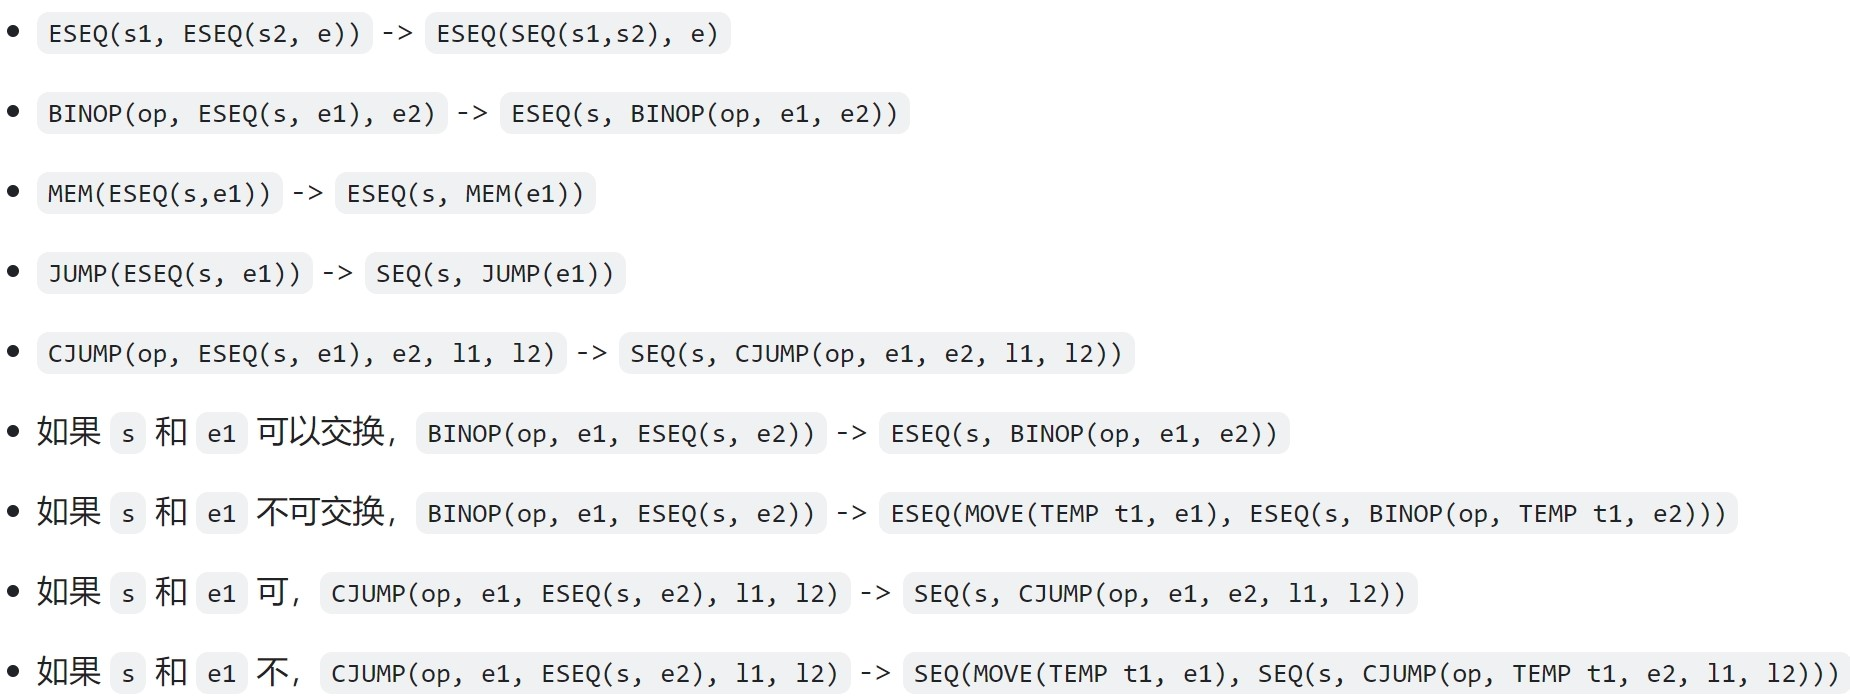
\includegraphics[width=\linewidth]{figures/irc1.png}
\end{figure}

\par \noindent Basic Blocks:一段代码中,只有一个入口点和一个出口点的连续代码块。Trace: 可以连续执行的基本块序列。
计算 trace:1. 某个 basic block 开始,往后继节点遍历,标记每个被访问的 basic block 并将其附加到当前 trace 中;
2. 当到达某 basic block 其后继节点均已标记,这个 trace 就算完了。
计算新的 trace:选择一个未标记的 basic block 作为下一个 trace 的起点。
全局终止条件:不断迭代、 直到所有的 basic blocks 都被标记。
(性质)每个 trace 都是无环的。

\par \noindent 调整 \texttt{CJUMP} 后面紧跟的标签:a. 如果跟着的标签是 true 标签,互换 true 和 false 标签,并对条件取反;
b. 如果跟着的标签是 false 标签,什么都不做;
c. 如果跟着的标签既不是 true 标签,也不是 false 标签,替换 \texttt{CJUMP(cond, a, b, lt, lf)} $\rightarrow$
\texttt{CJUMP(cond, a, b, lt, lf'); LABEL lf'; JUMP(NAME lf)}。
% ======================================================
\section{Instruction Selection}
\label{section:instruction-section}
% !TEX root = ./main.tex
% Instruction Selection
% ======================================================
\par \noindent 基于树的模式匹配:
中间表示树上的一个部分作为一个单元,对应可供选择的某条汇编指令。将指令选择问题转变为图的覆盖问题(选择代价最小的覆盖):
(虚拟寄存器和临时变量不会生成对应的汇编指令)

\begin{figure}[H]
    \centering
    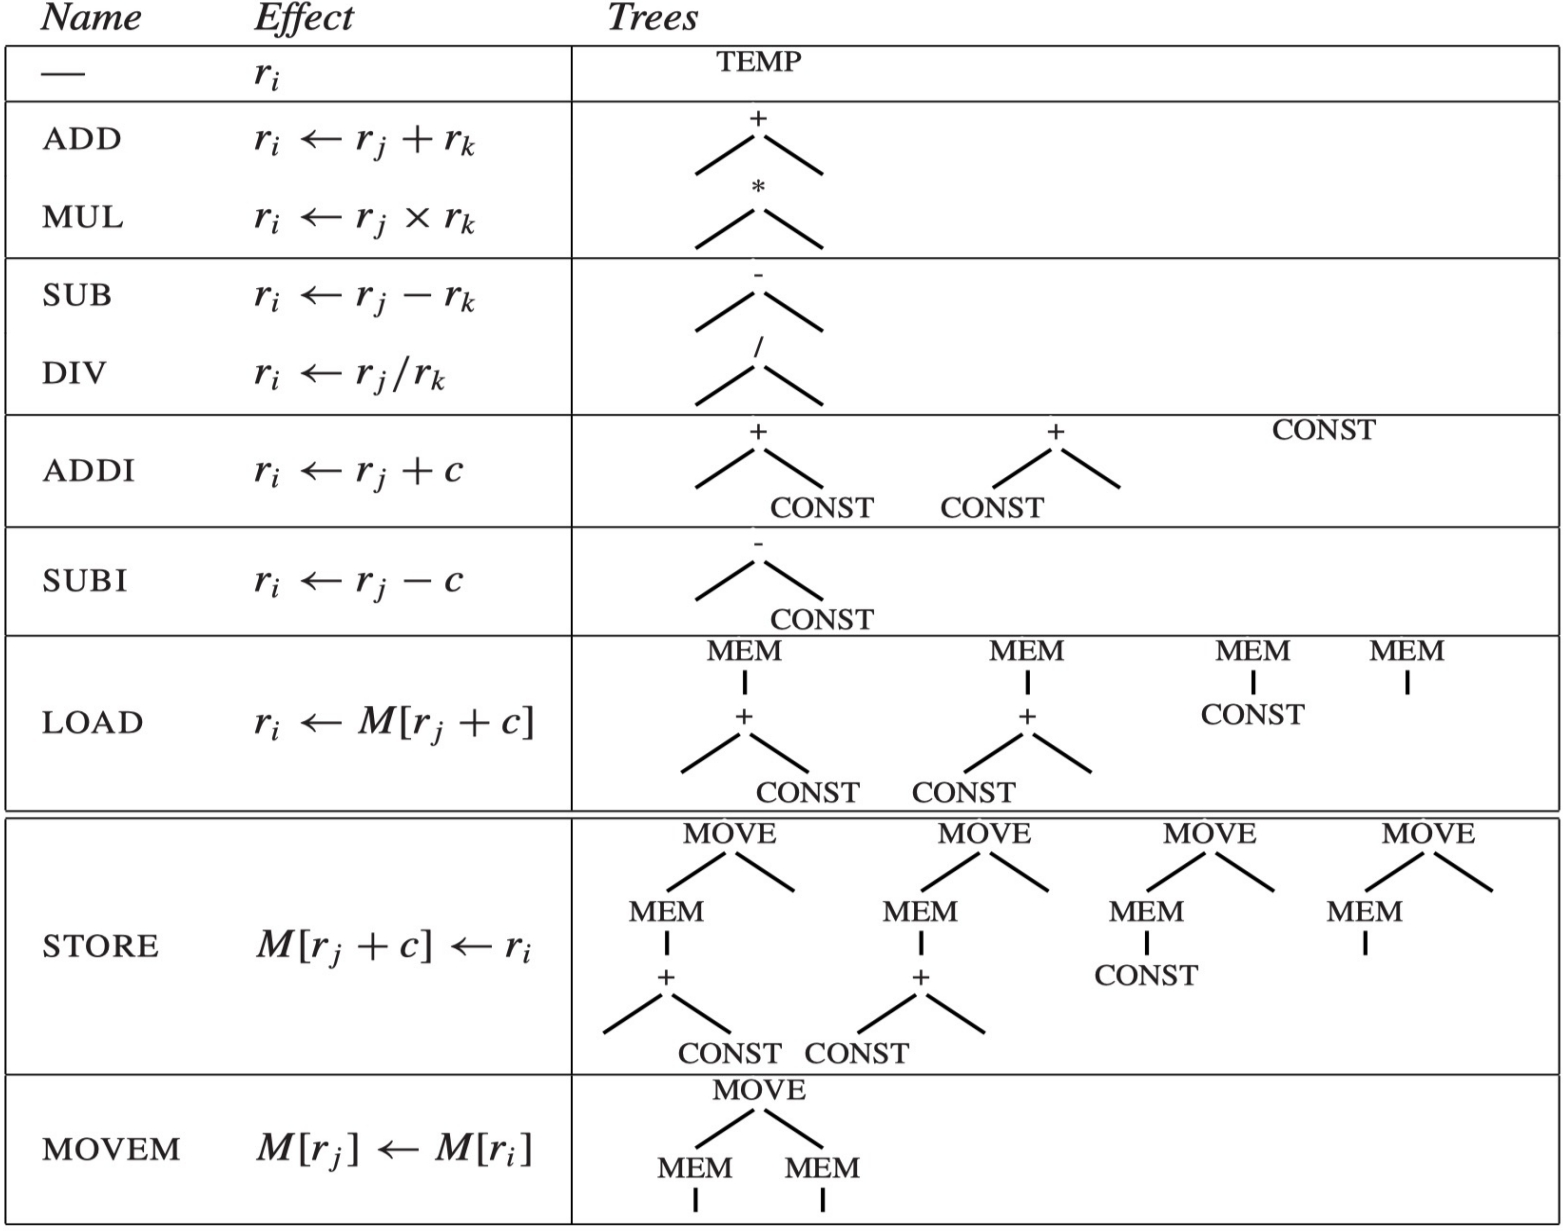
\includegraphics[width=\linewidth]{figures/is1.png}
\end{figure}

\par \noindent Optimum Tiling: 全局最优,整体代价最低;Optimal Tiling: 局部最优,每个片段最优但整体不一定最优。

\par \noindent Maximal Munch 算法:找到 Optimal Tiling。这是一个贪心算法,认为选择越大(节点数越多)的 Tile 导致的代价越小。
遇到相同大小的 Tile 任选其一。
从 IR 树的根节点开始,每次选择能够覆盖当前节点的最大图块,这将把原先的 IR 树分割为若干子树。
对每个被分割出的子树,重复相同的算法。
在完成 Tile 的放置后,以相反的顺序生成指令(从叶节点向根节点生成)。

\par \noindent 动态规划:找到 Optimum Tiling(一旦最小代价 tiling 的所有子树都被找到,那么根据这些子树的代价可以确定根节点的最小代价 tiling)。
自下而上地计算每个节点的最小成本。对于每个节点,首先计算其子节点的最小总成本 Tiling。每个节点的成本 := 所选 Tile 的成本 + 产生的子树的成本。
对于节点 $x$,定义 $f(x)$ 为以 $x$ 为根节点的树的 Optimal Tiling 的总成本,$f(x)$ 以下面的公式计算: 
\vspace{-10pt}
$$
f(x) = \min_{\forall T\text{ covering }x}\left( \text{cots}(T) + \sum_{\forall \text{ child }y\text{ of tile }T}f(y) \right)
$$
\vspace{-15pt}
\par \noindent 当整棵 IR 树的根节点的最小代价被找到,根据 IR 树的所有结点的代价状态,可以确定指令的选择(这个过程被称为 instruction emission),方法为:

\begin{figure}[H]
    \centering
    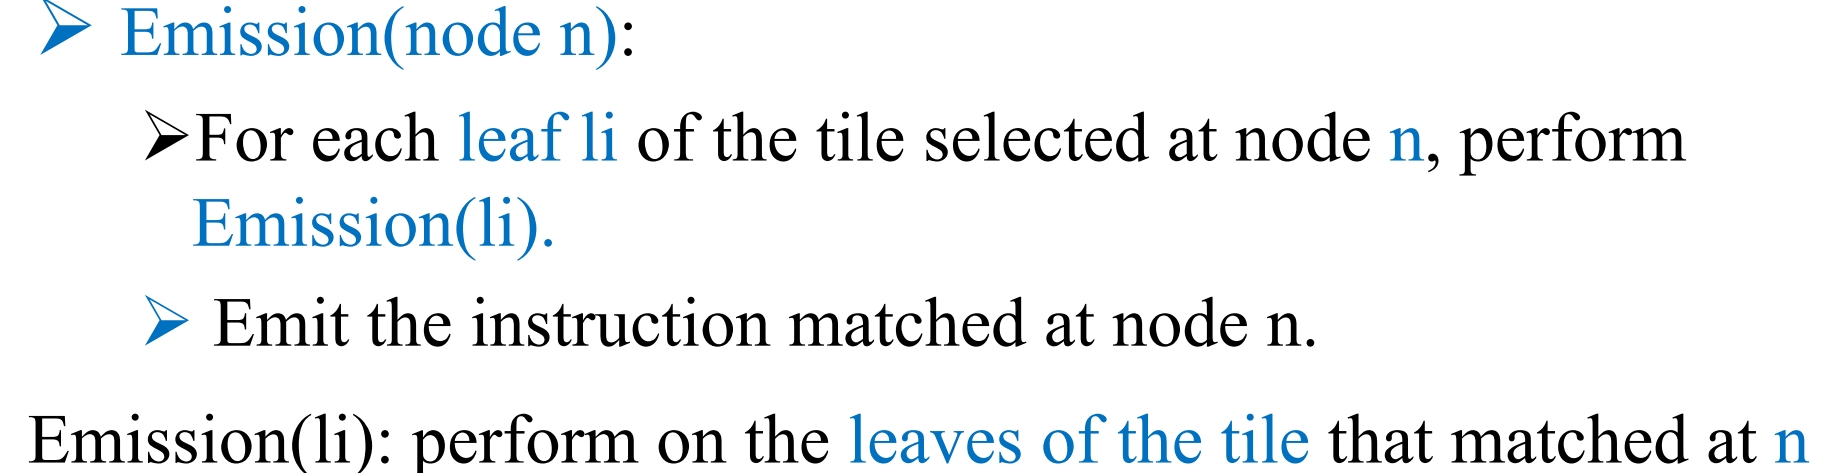
\includegraphics[width=0.8\linewidth]{figures/is2.png}
\end{figure}

\par \noindent Tree Grammar:对于 CISC 架构,对代码生成器中的 tile 进行硬编码可能很繁琐且 error-prune,
使用 Tree Grammar(一种特殊的 CFG)来描述图块,将指令选择简化为 parse 问题,使用动态规划算法进行 parse。
Tile 之间的关系被编码为重写规则,每个规则包括:Tree Grammar 中的产生式、Tile 的代价、翻译模板。
Tree Grammar 可能有二义性(有许多不同的指令序列实现相同的表达式),因此使用 DP。

% ======================================================
\par \noindent CISC 架构的其他问题【解决方案】:
1. 寄存器较少【不限制生成 TEMP 节点,假设寄存器分配能完成分配工作】;
2. 寄存器分类【将操作数显示地传送到相应的寄存器中】;
3. 两地址指令【增加一条额外的传送指令】;
4. 算数运算可以访问存储器【指令选择阶段将每一个 TEMP 节点转化成一个寄存器引用】;
5. 若干种寻址模式【这是优点,破坏寄存器少;指令代码短】;
6. 变长指令【不管】;
7. 副作用指令【三种解决办法:忽略地址自增指令、在采取树型匹配的代码生成器的上下文中使用特别方式匹配特殊的习惯用法、使用完全不同的指令算法,基于 DAG 样式】。
% ======================================================
% reference: https://github.com/Tian42chen/Transcription-Malfunctioned/blob/main/Compiler%20Principle/content/CP-CheatSheet9.tex

% ======================================================
\section{Liveness Analysis}
\label{section:liveness-analysis}
% !TEX root = ./main.tex
% Liveness Analysis
% ======================================================
\par \noindent 称变量 \texttt{x} 在语句 \texttt{s} 中是活跃的,iff:
存在使用变量 \texttt{x} 的语句 \texttt{s'} 且
有一条从 \texttt{s} 到 \texttt{s'} 的路径,该路径中没有对 \texttt{x} 的赋值/定义。
\par \noindent 称变量 \texttt{x} 在边 E 上是活跃的,iff:$x \in \text{use}(s')$ 且
有一条经过 E,到 \texttt{s'} 的路径,并且该路径中的所有节点的 $\text{def}()$ 均不包括 \texttt{x}。

\par \noindent 判断变量在某个位置是否活跃:不可判定。保守的近似算法:
\vspace{-10pt}
$$
\begin{array}{rl}
    \text{in}(n)  &= \text{use}(n) \cup (\text{out}(n) - \text{def}(n)) \\
    \text{out}(n) &= \bigcup_{s \in \text{succ}(n)} \text{in}(s)
\end{array}
$$
\vspace{-15pt}
\par \noindent 初始条件:$\text{in}(n) = \varnothing$,$\text{out}(n) = \varnothing$;迭代直到不动点。
一定收敛的原因:单调有界定理。
求并集: $\mathcal{O}(N)$,每一次迭代:$\mathcal{O}(N^2)$,至多迭代:$\mathcal{O}(2N^2)$;总复杂度 $\mathcal{O}(N^4)$。
如果选择合适的顺序,实际运行时间介于 $\mathcal{O}(N)$ 与 $\mathcal{O}(N^2)$。

\par \noindent 优化:倒序,从后往前,对每个节点先计算 out 再计算 in。

\par \noindent 静态活跃性:存在一条控制流路径;动态活跃性:运行时。动态活跃 $\Rightarrow$ 静态活跃。
静态活跃性是一种保守的近似估计,它认为所有分支都会被执行。上面的算法是一种静态活跃性分析,这体现在第二个式子中。

% ======================================================
\section{Register Allocation}
\label{section:register-allocation}
% !TEX root = ./main.tex
% Register Allocation
% ======================================================
\par \noindent 图着色算法。寄存器数量 $=K$,node with significant degree = 这个节点在相关图中有 $\geq K$ 条边,反之为 significant。

\par \noindent 相关图中用虚线连接的节点表示这两个寄存器 \texttt{a, b} 存在 \texttt{a := b},并且不冲突,他们是 coalesce 的候选节点(move-related)。

\par \noindent 1. 选择一个 insignificant 节点,将其从图中移除,加入栈中;
如果没有符合条件的节点,则选择一个 significant 节点,将其移除,加入 remove 列表中,然后加入栈中(optimistic coloring)。
2. 重复第一步,直到图为空。
3. 从栈中弹出节点,将其着色,直到所有节点都被着色。
4. 如果遇到无法着色的节点,则意味着要做 actual spill,重新生成代码,生成相关图,重复。

\begin{figure}[H]
    \centering
    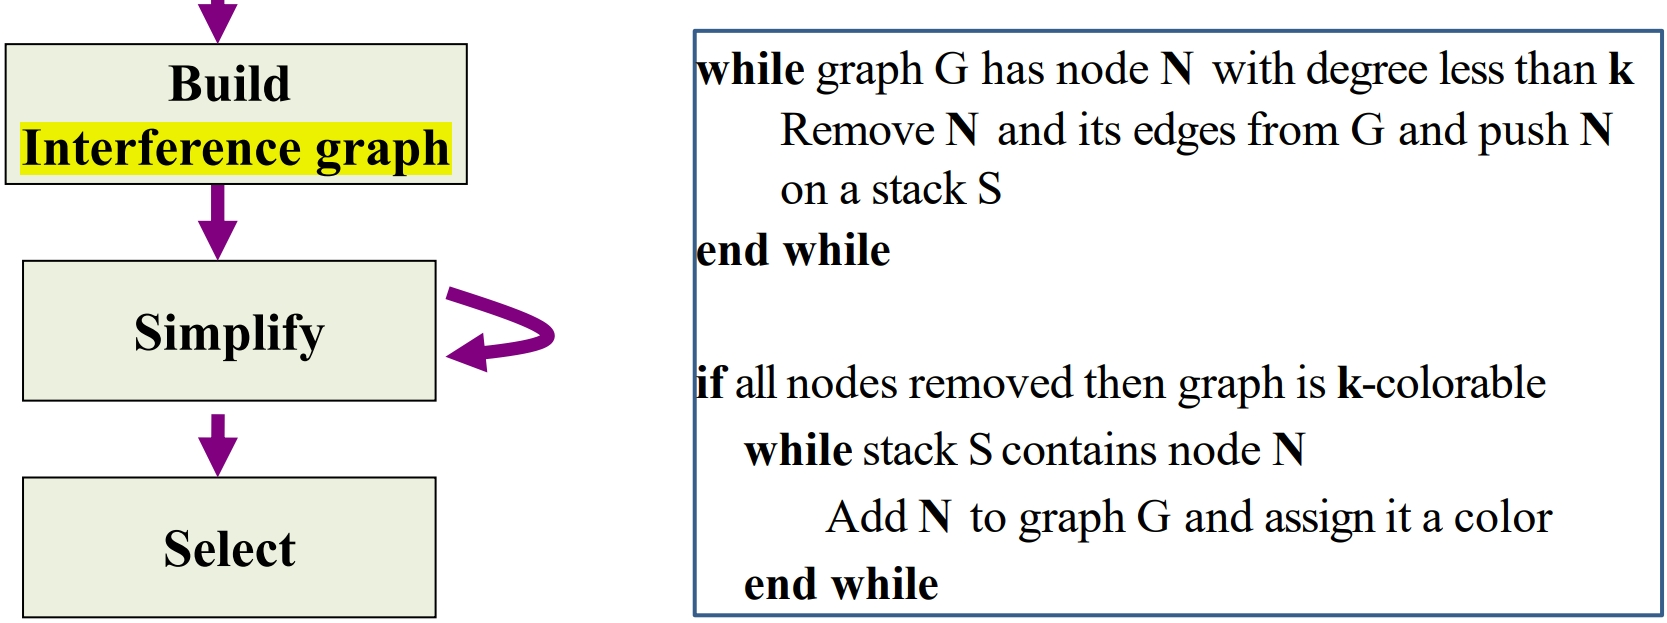
\includegraphics[width=0.8\linewidth]{figures/ra1.png}
\end{figure}

\par \noindent 上面的算法可能会失效,需要 coalescing。保守的 coalesce 对两个候选节点是否能够合并的判据(二选一):
1. (Briggs:avoid creation of high-degree $(\geq K)$ nodes)如果合并后的节点拥有小于 $K$ 个 significant 邻居;
2. (George)如果合并前,a 的每一个邻居要么是 b 的邻居,要么是 insignificant,则可以合并 ab。

\begin{figure}[H]
    \centering
    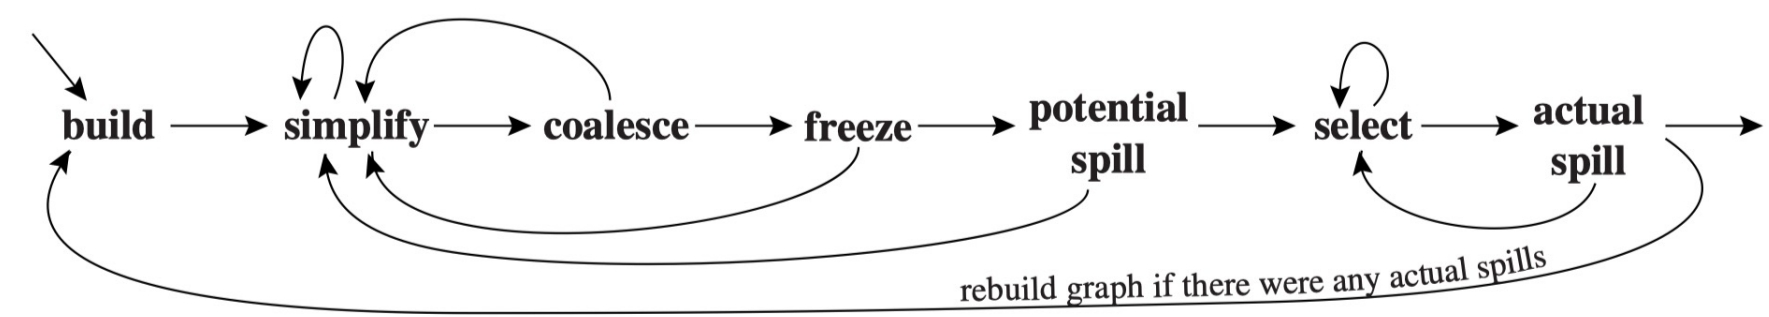
\includegraphics[width=0.8\linewidth]{figures/ra2.png}
\end{figure}

\par \noindent 1. build:构建相关图(包括虚线);
2. simplify:将图中 insignificant、non-move-related 节点移除,加入栈中;
3. coalesce:合并节点,重复 2 和 3 直到所有节点都是 significant 或者 move-related(但不能合并);
4. freeze:将低度的 move-related 节点视为 non-move-related,返回 2;
5. spill:选择高度节点进行 spill,将其移除,加入 remove 列表中,然后加入栈中(optimistic coloring);
6. select:从栈中弹出节点,将其着色,直到所有节点都被着色;
7. 如果遇到无法着色的节点,则意味着要做 actual spill,重新生成代码,生成相关图,重复。

\par \noindent Spill priority $= \frac{(\text{Use+Def Outside loop}) + 10 \times (\text{Use+Def inside loop})}{\text{Degree}}$(经验公式),
spill 这个数值最低的节点。

\par \noindent 预着色节点:不能被 simplify,不能被 spill。此时着色算法的目的是删除除了预着色节点以外的所有节点。

\par \noindent Callee-save register:Any variable that is live across several procedure calls;
Caller-save register:A local variable or compiler temporary that is not live across any procedure call。
% ======================================================
\section{Garbage Collection}
\label{section:garbage-collection}
% !TEX root = ./main.tex
% Garbage Collection
% ======================================================
\par \noindent 不可判定问题,使用可达性作为近似。
使用有向图,节点为程序变量和堆分配的记录,边为指针。
有向图的根节点是程序变量(寄存器、堆栈上的局部变量/形参、全局变量)。

\par \noindent \textbf{Mark-Sweep} Mark:从根节点出发遍历所有可到达的节点;Sweep:线性扫描扫描整个堆,将未标记的节点放入 free list。
垃圾回收后,程序恢复执行;每当在堆上分配新记录时,从 freelist 中获取一条记录;当 freelist 为空时,再次执行垃圾回收。
假设 $H$ 为堆大小,$R$ 可达数据数,一次 GC 的总时间 $c_1 R + c_2 H$,摊还时间为 $\frac{c_1 R + c_2 H}{H - R}$。
优化:显式栈:减少 DFS 递归调用的内存开销;指针反转:访问子节点时反转指针,以便回溯。
% 指针反转的具体算法不考
\par \noindent 优点:
1. 垃圾不多时效率高;
2.能够处理循环引用;
3. 对象/记录在 GC 期间不会移动。
缺点:
1. 垃圾多时效率低;
2. GC 时必须暂停程序执行;
3. 导致堆中的碎片化(这会导致缓存未命中、页抖动、更复杂的内存分配)。

\par \noindent \textbf{Reference Counting} 跟踪指向每个对象的指针数量(引用计数);每当建立新引用时,递增引用计数,反之递减;
当引用计数变为 0 时,对象是无法访问的垃圾。
优点:
1. GC 与程序执行交错,是 incremental overhead,没有 stop-and-collect 效应;
2. 相对容易实现;
3. 可与手动内存管理共存;
4. Spatial locality of reference is good(Access pattern to virtual memory pages no worse than the program, so no excessive paging);
5. 可以立即重用释放的单元。
缺点:
1. 无法处理循环引用;
2. 每次引用计数变化都需要更新计数器,开销大。

\par \noindent \textbf{Copying} 使用两个堆:from-space 和 to-space。当 from-space 耗尽时,遍历 from-space,将所有可达节点复制到 to-space;当下一次耗尽时,反转。
Pointer Forwarding:找到一个可达的记录时,将其复制到 to-space,并在 from-space 中存储指向新副本的转发指针。
\par \noindent Cheney’s Algorithm:将 to-space 划分为三个连续区域,使用 BFS 遍历可达数据,从 from-space 复制到 to-space。

\begin{figure}[H]
    \centering
    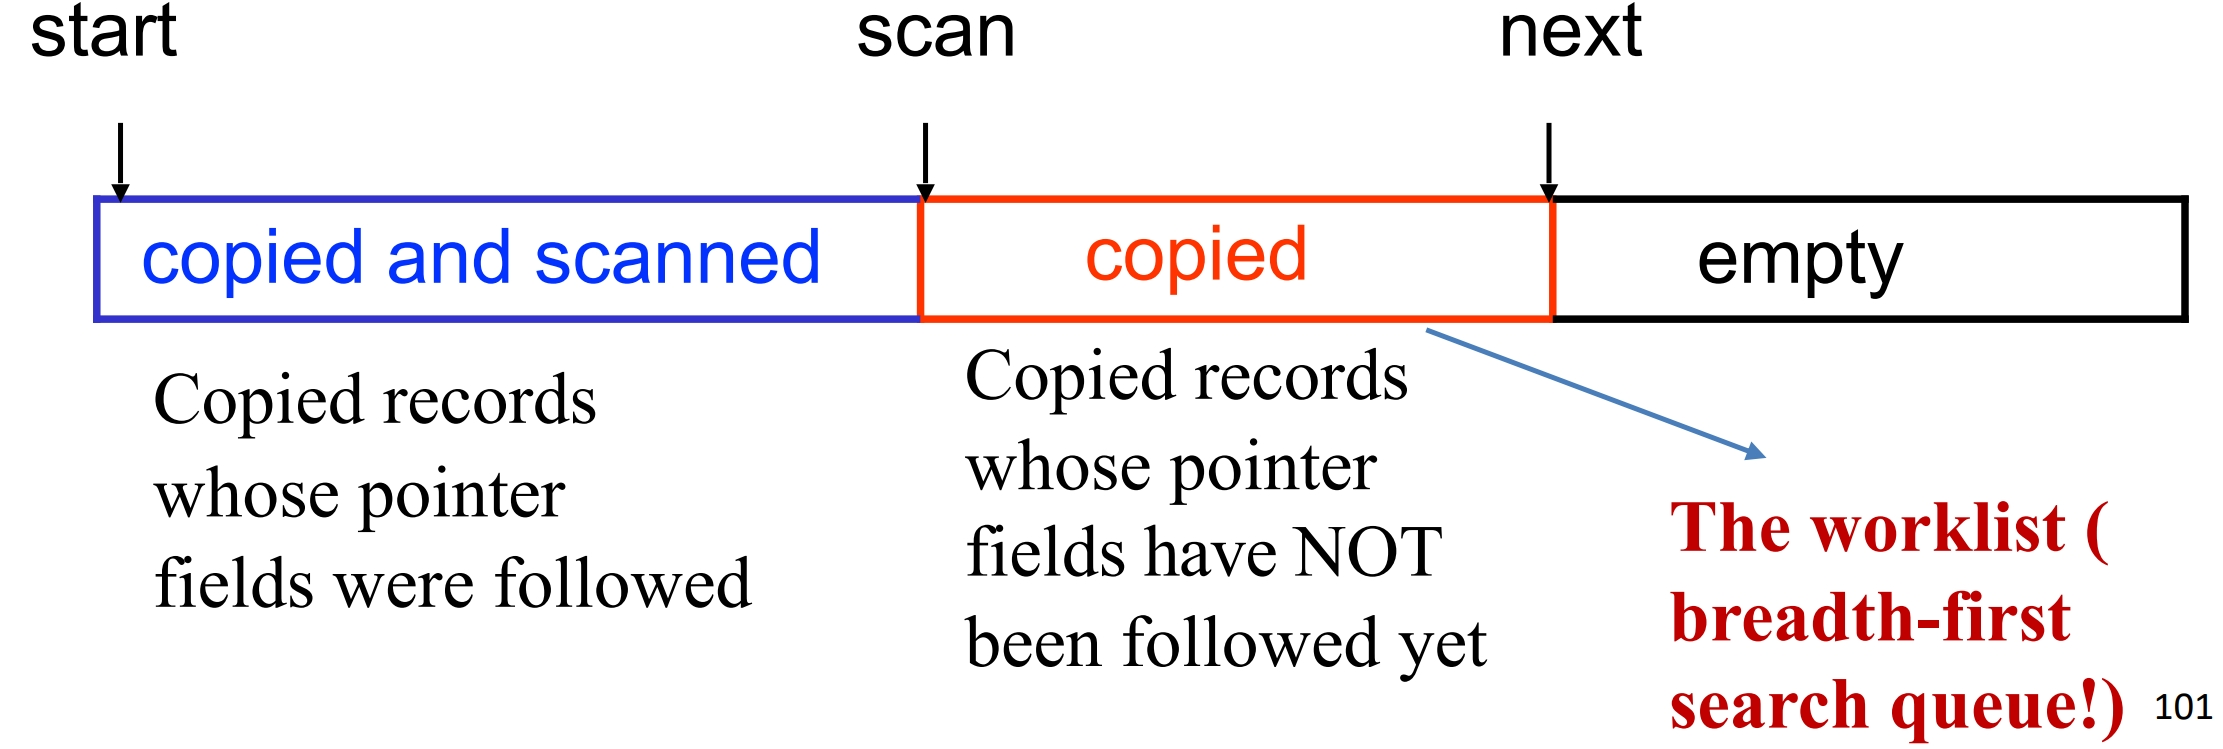
\includegraphics[width=0.8\linewidth]{figures/gc1.png}
\end{figure}

\begin{figure}[H]
    \centering
    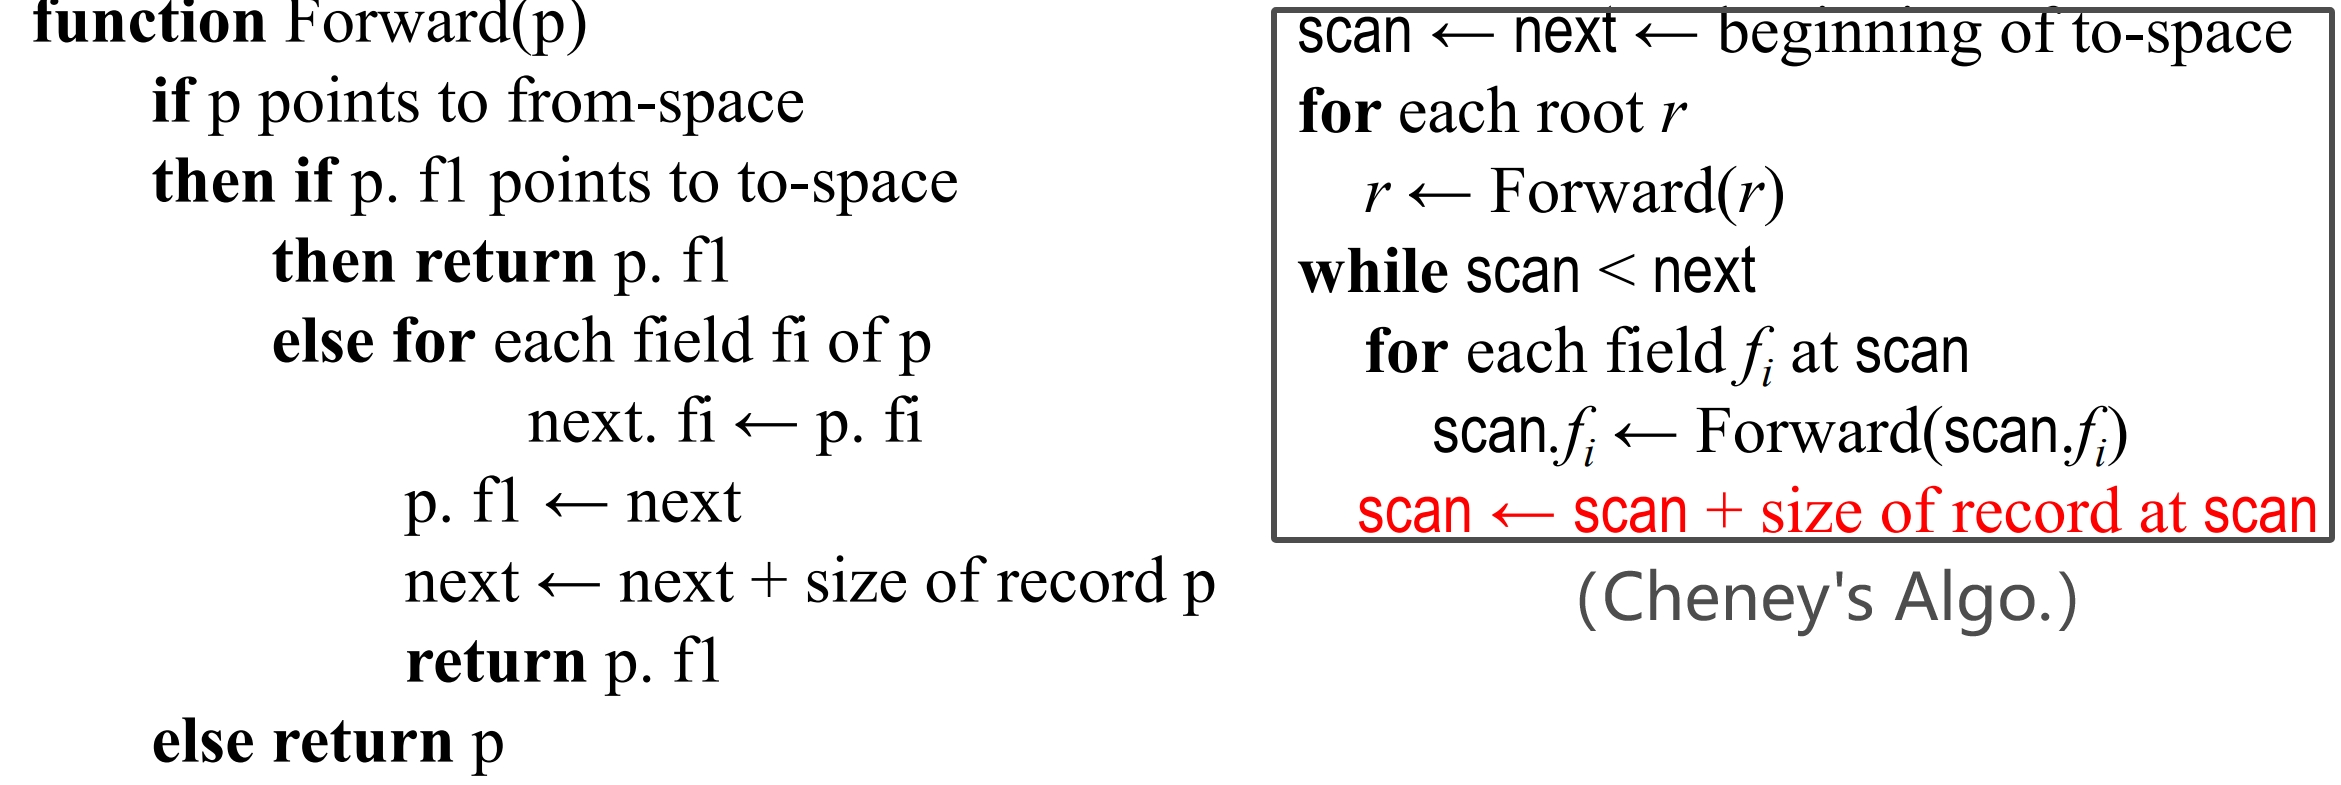
\includegraphics[width=0.8\linewidth]{figures/gc2.png}
\end{figure}

\par \noindent 改进 BFS 带来的局部性差的问题:使用 BFS,但是每当复制对象时,查看是否可以在它附近复制一些子项。

\par \noindent 优点:
1. 简单,无需栈或指针反转;
2. 运行时间与活跃的对象数量成正比;
3. 空闲空间连续;
4. 自动压缩消除碎片化;
5. 是许多后续算法的基础。
缺点:
1. 一半内存被浪费;
2. 局部性差(Cheney’s Algorithm);
3. 需要精确的类型信息(指针或非指针)。

\par \noindent 编译器需要为 GC :
1. Generating code that allocate records;
2. Describing locations of roots for each garbage collection cycle;
3. Describing the layout of data records on the heap;
4. Generating instructions to implement a read or write barrier(for some versions of incremental collection);
5. \dots

\par \noindent \textbf{Fast Allocation (for Copying Collection)} 
分配记录的过程:
1. Call the allocate function;
2. Test next + N < limit ? (If the test fails, call GC);
3. Move next to result;
4. Clear M[next], M[next+1], ..., M[next + N - 1];
5. next <- next + N;
6. Return from the allocate function。
这里的步骤 2 和 5 无法消除,通过在寄存器中保留 next 和 limit,步骤 2 和 5 总共可以在 3 条指令中完成,
分配记录的成本可以降低到大约 4 条指令,然后进行 GC。

\par \noindent Describing Data Layouts:类描述符生成,语义分析阶段。

\par \noindent Exact Root Description (Pointer Map),包含栈上的指针和 callee-saved 寄存器中的指针。
在何处插入 Pointer Map 取决于 GC 在何时触发:分配时:在 \texttt{alloc\_record}之前插入;递归调用时:插入所有函数调用。
To find all the roots, the collector starts at the top of the stack and scans downward.
1. Each return address keys the pointer-map entry that
describes the next frame;2.In each frame, the collector marks (or forwards, if copying collection) from the pointers in that frame.
Callee-save registers need special handling, the pointer map for g must describe 
which of its callee-save registers contain pointers at the call to h and which are “inherited” from f.

\par \noindent Derived Pointers:\texttt{t1 <- a - 2000; t2 <- t1 + i; t3 <- M[t2]},
We say that t1 is derived from the base pointer \texttt{a}. 
The pointer map must identify each derived pointer and tell its base pointer.
When the collector relocates \texttt{a} to address \texttt{a'}, it must adjust \texttt{t1} to point to address \texttt{t1 + a' - a},
\texttt{a} must remain live as long as \texttt{t1} is live.
% ======================================================
\section{Object-Oriented Languages}
\label{section:object-oriented-languages}
% !TEX root = ./main.tex
% Object-Oriented Languages
% ======================================================
\subsection*{Single Inheritance}

\begin{figure}[H]
    \centering
    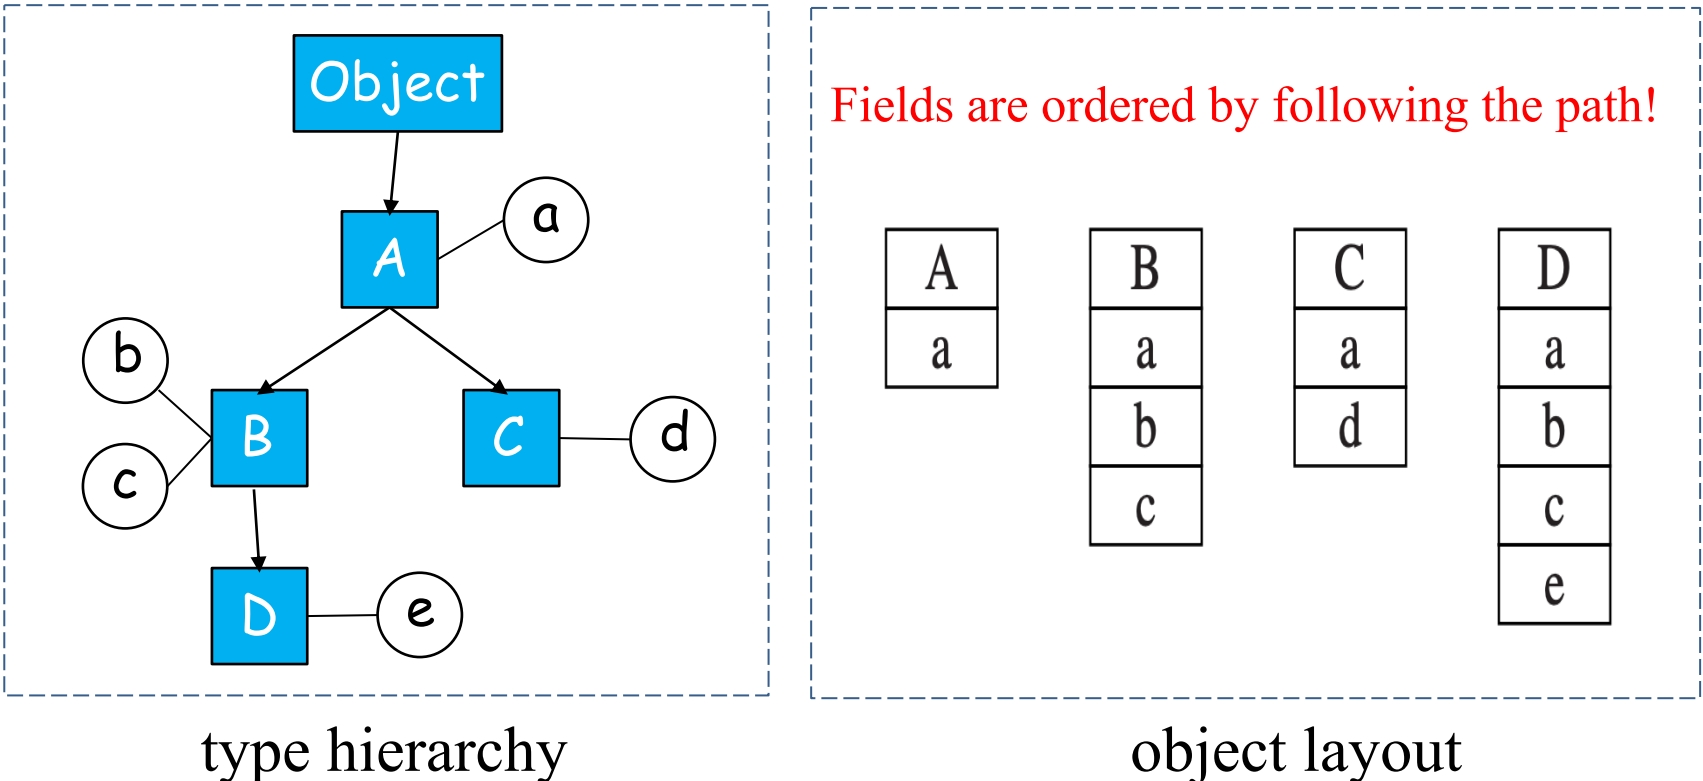
\includegraphics[width=0.40\linewidth]{figures/oop1.png}
    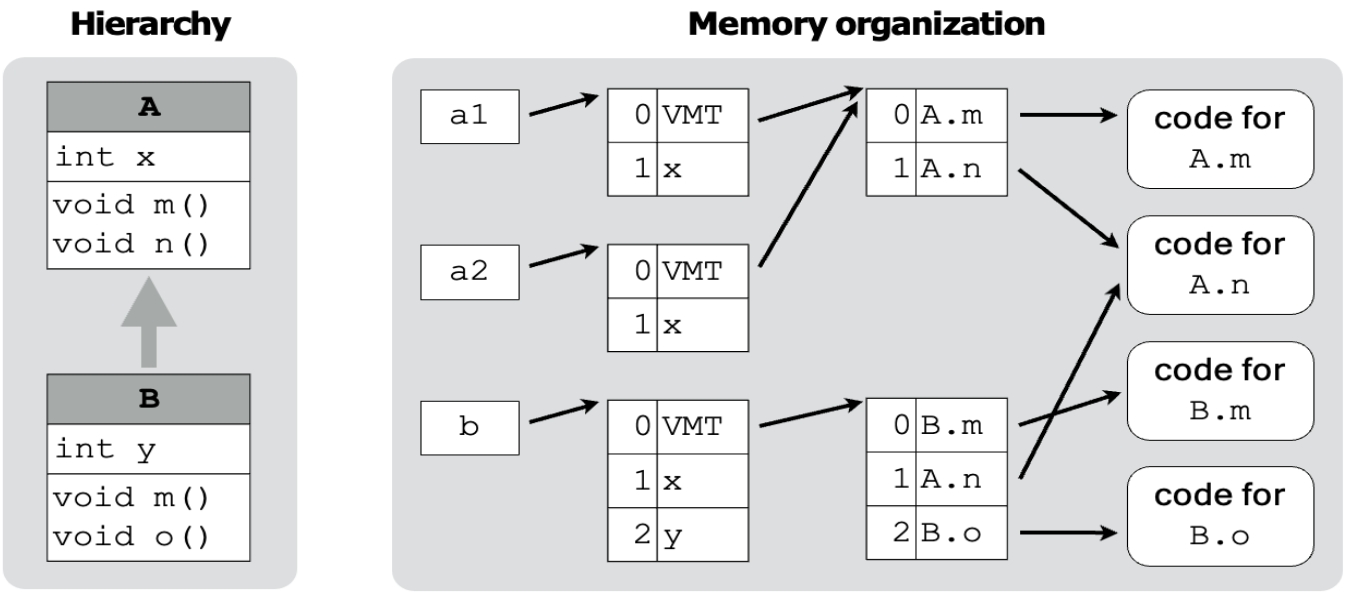
\includegraphics[width=0.58\linewidth]{figures/oop2.png}
\end{figure}

\par \noindent \textbf{Field layout}:继承的字段以相同的顺序放在类描述符头部。

\par \noindent \textbf{Method dispatch}(= generating method calls):每个类描述符都包含指向其父类的指针,以及方法实例列表。
\par \noindent 对于静态方法:调用 \texttt{c.f()} 时在类 C 中搜索方法 f,如果找不到 – 搜索 C 的父类,依此类推。
\par \noindent 对于动态方法:使用 dispatch vector(aka virtual table, vtable),记录所有方法的地址。
调用 \texttt{c.f()} 时从 c 中偏移量为 0 处获取类描述符 d,从 d 偏移 f (常数)中获取方法实例指针 p。

\subsection*{Multiple Inheritance}

\par \noindent \textbf{Field layout}:图着色算法,每个类的字段按照其在继承图中的位置着色,颜色代表其偏移量。
如果不同字段在同一个类型里出现了,那么它们就不能染成同一个颜色。优化:由于类型数远小于对象数,偏移量在类描述符中,而非直接在对象中。

\par \noindent \textbf{Method dispatch}:图着色算法,同上。

\par \noindent \textbf{Dynamic Linking Class}:无法使用图染色算法,解决方案是哈希表。
为每个类描述符构建哈希表:1. Ftab(字段表):包含字段偏移量和方法代码地址;2.Ktab(键表):包含字段/方法名称。
获取字段 b 的步骤:
1. 从偏移量 0 处获取类描述符;
2. 从 $\text{Ktab} + \text{hash}_b$ 处获取字段名;
3. 比较字段名和输入名;
4. 若相等,从 $\text{Ftab} + \text{hash}_b$ 处获取字段偏移量,假设为 $2$;
5. 从 $\text{object} + 2$ 处获取字段。

\par \noindent \textbf{Membership test}:每一个类描述符存储一个 display:类嵌套深度限制为某个常量(例:20),在每个类描述符中保留一个 20 字长的块。
给每个类指定一个数字标识符:

\begin{figure}[H]
    \centering
    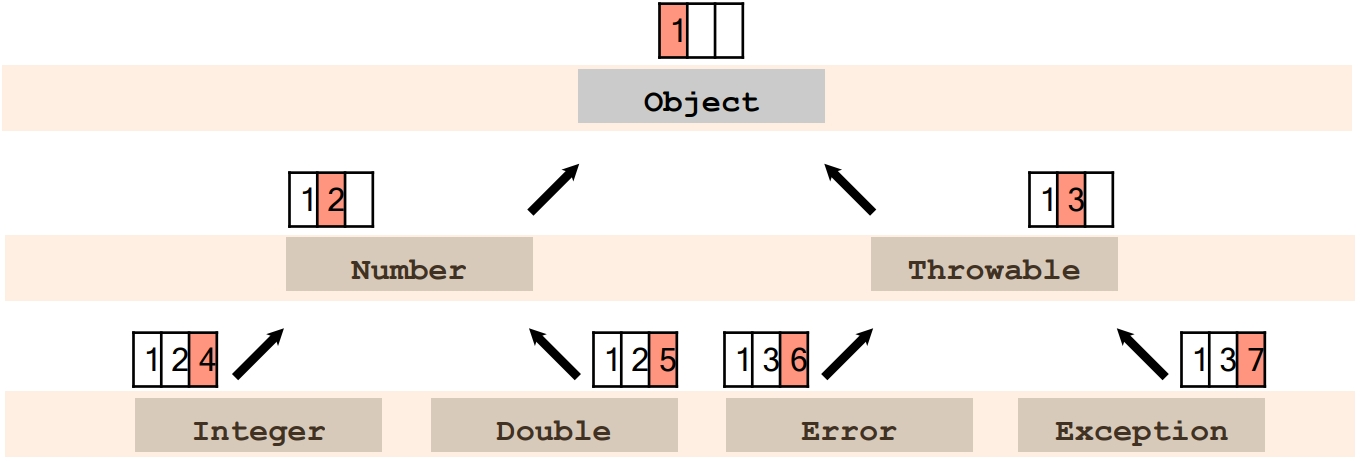
\includegraphics[width=0.8\linewidth]{figures/oop3.png}
\end{figure}

\par \noindent 通过类型检查可以实现私有方法/成员变量。类型转换到超类(upcast)是安全的,但是转换到子类(downcast)是不安全的。
% ======================================================
\section{Loop Optimizations}
\label{section:loop-optimizations}
% !TEX root = ./main.tex
% Loop Optimizations
% ======================================================
\par \noindent 支配节点(Dominators):若 $d$ 支配 $n$,则从流图的入口 $s_0$ 到节点 $n$ 的每条路径都经过节点 $d$。
计算支配 $n$ 的所有节点 $D[n]$:$D(n) = \{n\} \cup \bigcap_{p \in \text{pred}(n)} D[p]$,初始条件:$D[s_0] = \{s_0\}$。
\par \noindent 直接支配结点(immediate dominator):支配节点集合中除了 $n$ 本身的最接近 $n$ 的节点。
\par \noindent 支配节点树(dominator tree):树中一个节点的子节点是该节点的直接支配节点。每个结点只支配它和它的后代结点。

\par \noindent Back Edge:当 $h$ 支配 $n$ 时从 $n$ 到 $h$ 的边。
Back Edge $n \rightarrow h$ 的自然循环是满足以下条件的节点 $x$ 的集合:1.$h$ 支配 $x$;2. 有一条从 $x$ 到 $n$ 的路径不包含 $h$。
自然循环满足性质:1. 有唯一的入口结点,称为首结点(header);2. 首结点支配循环中的所有结点;3. 循环中至少有一条返回首结点的路径;
4. 除非两个自然循环的首结点相同,否则,它们要么互不相交,要么一个完全包含在另外一个里面。
\par \noindent 循环嵌套树(Loop-Nest Tree):树的叶节点是最内层循环。构造:
1. 画出支配节点树;
2. 找到所有自然循环,并找到所有循环首结点;
3. 对于每个循环首结点 $h$,将 $h$ 的所有自然循环合并为一个循环 $\text{loop}[h]$,循环中的节点写在第二行,首节点写在第一行;
4. 如果 $h_2$ 在循环 $\text{loop}[h_1]$ 中,那么 $h1$ 在循环嵌套树中高于 $h_2$。

\begin{figure}[H]
    \centering
    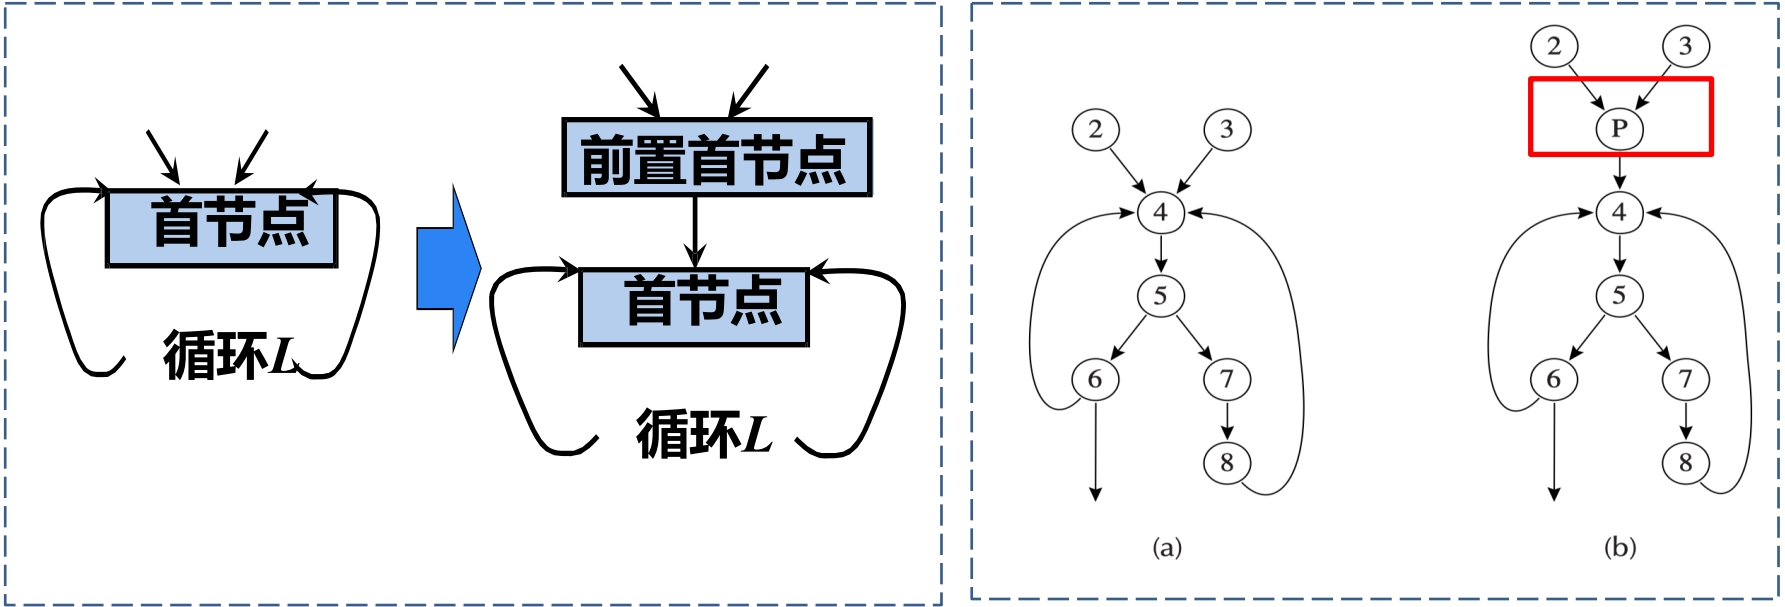
\includegraphics[width=0.8\linewidth]{figures/loop1.png}
\end{figure}

\par \noindent 循环不变式(Loop Invariant):在循环中,每次迭代都保持不变的量。循环不变式的生成:
表达式 \texttt{x := v1 op v2} 是循环 $L$ 中的不变式,当且仅当:(基础情况)it’s a constant 或者 
it’s a variable use, all of whose defs are outside of $L$;
(归纳情况)it’s a pure computation all of whose arguments are loop-invariant 或者
it’s a variable use with only one reaching def, and the rhs of that def is loop-invariant。

\par \noindent 提升(Hoist) \texttt{d : t <- a op b} 到循环的前置首节点(preheader)末尾的条件:
1. $d$ dominates all loop exits where $t$ is live-out(很可能阻止许多计算从 while 循环中提升);
2. and there is only one definition of $t$ in the loop;
3. and $t$ is not live-out of the loop preheader (that is, $t$ is not live before the loop)。
如果 \texttt{d : t <- a op b} 可能引起某种算术异常或产生其他副作用,则需要修改这些规则。
% ======================================================
\end{multicols}
\end{document}
% ======================================================
% reference: 浙江大学编译原理课程课件,pyaoaa at zju.edu.cn
% ======================================================